\documentclass{article}
\usepackage{fullpage}

\usepackage{amsmath,amsthm,amssymb}
\usepackage[utf8x]{inputenc}
\usepackage{hyperref}

\newtheorem{lemma}{Lemma}
\newtheorem{theorem}{Theorem}
\newtheorem{corollary}{Corollary}
\newtheorem{proposition}{Proposition}
\newtheorem{conjecture}{Conjecture}
\newtheorem{wellknown}{Standard Knowledge}
\newtheorem{problem}[conjecture]{Problem}
\theoremstyle{definition}
\newtheorem{definition}{Definition}
\newtheorem{sdef}{Standard Term}

\newcommand{\N}{\mathbb{N}}
\newcommand{\NZ}{\N_0}
\glossary{$\NZ$: natural numbers including 0}
\newcommand{\Z}{\mathbb{Z}}
\newcommand{\Q}{\mathbb{Q}}
\newcommand{\QP}{\mathbb{Q}_+}
\newcommand{\R}{\mathbb{R}}
\newcommand{\C}{\mathbb{C}}
\newcommand{\RP}{\mathbb{R}_+}
\newcommand{\RI}{\R_{>1}}
\newcommand{\RII}{\R_{\ge 1}}
\newcommand{\then}{\Longrightarrow}
\newcommand{\wo}{\setminus}
\newcommand{\propref}[1]{proposition \ref{#1}}
\newcommand{\defref}[1]{definition \ref{#1}}
\newcommand{\rh}{\varrho}
\newcommand{\eps}{\varepsilon}
\newcommand{\ph}{\varphi}
\newcommand{\sexp}{\operatorname{sexp}}
\newcommand{\slog}{\operatorname{slog}}
\newcommand{\spow}{\operatorname{spow}}
\newcommand{\rsexp}{\sexp^{\mathfrak{R}}}
\newcommand{\rslog}{\slog^{\mathfrak{R}}}
\newcommand{\rusexp}{\sexp^{\mathfrak{R}^+}}
\newcommand{\ruslog}{\slog^{\mathfrak{R}^+}}
\newcommand{\msexp}{\sexp^{\mathfrak{M}}}
\newcommand{\mslog}{\slog^{\mathfrak{M}}}
\newcommand{\ksexp}{\sexp^{\mathfrak{C}}}
\newcommand{\kslog}{\slog^{\mathfrak{C}}}
\newcommand{\isexp}{\sexp^{\mathfrak{I}}}
\newcommand{\islog}{\slog^{\mathfrak{I}}}

\newcommand{\mt}[1]{\quad\mbox{#1}\quad}
\newcommand{\abs}[1]{\left|#1\right|}
\newcommand{\I}{\mathrm{i}}
\newcommand{\di}{\mathrm{d}} %*d*elta of *i*ntegration

%commands by Kouznetsov begin
\usepackage{graphics}
\usepackage{rotating}
\newcommand \sx {\scalebox}
\newcommand \rme {\mathrm{e}}
\newcommand \rot {\begin{rotate}}
\newcommand \ero {\end{rotate}}
\newcommand \rf[1] {(\ref{#1})}
\newcommand \iL[1] {~ \label{#1} ~~~[#1]}
\newcommand \ing {\includegraphics}
\newcommand \rmi {\mathrm{i}}
\newcommand \be {\begin{eqnarray}}
\newcommand \ee {\end{eqnarray}}
\newcommand \eL[1] {\iL{#1} \end{eqnarray}}
%commands by Kouznetsov end

\DeclareMathOperator{\id}{id} %locally with \operatorname{id}

% Local Variables:
% TeX-master: "main"
% End:


\author{Henryk Trappmann, Dmitrii Kouznetsov}
\title{5+ methods for real analytic tetration}

\numberwithin{equation}{section}
\begin{document}
\maketitle
\begin{abstract}
We feature different (mostly underexplored) methods for non-integer
iteration that accumulated over the past decades and
centuries. We show their relation if known and test them by
application to exponentials. 
We prove that the matrix power iteration, when applied to a fixed point, is the
(classic) regular iteration at that fixed point.
\end{abstract}

\section{Introduction}
Tetration in the sense of the fourth operation after addition,
multiplication and exponentiation is widely discussed in lay
mathematician communities. While multiplication is repeated addition
and exponentiation is repeated multiplication, one would define
tetration as repeated exponentiation: 
\newcommand{\tet}{\operatorname{[4]}}
\begin{align}\label{eq:tetration:informal}
  b\cdot n &:= \underbrace{b + \dotsb + b}_{n\times b}&
  b^n &= \underbrace{b\dotsm b}_{n\times b}&
  b\tet n &= \underbrace{b^{b^{.^{.^{.^b}}}}}_{n\times b}.
\end{align}
% It is a very natural procedure to define even higher operations along
% this scheme which is manifested in the orginal Ackermann function
% $\ph$ as defined by him in \cite{Ackermann:ReelleZahlen}  (to show that
% there are recursive functions that are not primitive recursive). Be
% however careful to not confuse this 3-argument function, which
% corresponds to our notation via $\ph(n,m,k)= n \operatorname{[k+1]}m$, with the
% later by R\'{o}zsa P\'{e}ter defined 2-argument Ackermann function,
% which serves simplification purposes \cite{Rozsa:Konstruktion}. 

As exponentiation is not associative there would be other ways to
bracket tetration and higher operations (for the use of arrows to
indicate different 
bracketings see Bromer \cite{bromer:superexponentiation}). In this article we are
however only concerned with right bracketed tetration
\eqref{eq:tetration:informal} and its extension to non-integer $n$.

The above formula \eqref{eq:tetration:informal} for tetration can be
inductively written as 
\begin{align}\label{eq:tetration:induction}
  b\tet 1 &= b &b\tet (n+1) &= b^{b\tet n}.
\end{align}
We want to keep this formula valid while extending from natural
numbers $n$ to non-integer $n$. Before we proceed with that let us see how
much we can extend tetration towards negative integers. The formula
\eqref{eq:tetration:induction} above is equivalent to $b\tet
(n-1)=\log_b (b\tet n)$. This gives then:
\begin{align}
  b\tet 0 &= 1 & b\tet (-1) &= 0
\end{align}
and $b\tet (-2)=\log_b(0)=-\infty$. So naturally we would restrict the
domain of any real-extended tetration to $(-2,\infty)$.

We assume that the reader is familiar with the behaviour of $x\tet n$
as $n\to\infty$. If not, it is a very illuminating exercise to plot the
graphs for several $n$. A proof for the following proposition can be
found in Knoebel's survey \cite{Knoebel:ExponentialsReiterated}.
\begin{wellknown}[Behaviour of $b\tet n$ for $n\to\infty$]
  The sequence $b_n= b\tet n$ converges for $e^{-e}\le b \le
  e^{1/e}$. The sequence $b_{2n}$ is strictly decreasing,
  $b_{2n+1}$ is strictly increasing and $b_{2n}>b_{2n+1}$ for $0<b<1$, both are
  convergent also for $0<b<e^{-e}$. The sequence $b_n$ is strictly
  increasing for $b>1$. 
\end{wellknown}
%TODO reference to Thron for general region of convergence.
The oscillating  behaviour of $b_n$ and the monotone
decrease of $x\mapsto b^x$ for $0<b<1$ is enough reason to exclude these bases
$b$ from our considerations. Indeed it can be shown (and be verified
by the reader) that using the later described method of regular
iteration (at the only real fixed point that $b^x$ got for these
bases) $b \tet x$ yields non-real complex values for most non-integer
$x$. Of course we also exempt the degenerated bases $0$ and $1$ from
our considerations.

The critical point 
\begin{align}
  \label{eq:eta}
  \eta:=e^{1/e}\approx 1.44466786
\end{align}
will divide most of the later featured methods. Some of them only work for $1<b<\eta$ or others work only for
$b>\eta$, see the table at the end of the article. This has to do
with the dependence of some methods on fixed points $z_0 = b^{z_0}$, see
knowledge \ref{wk:exponential:fixedpoint:real}. 

As the base $b$ occurs always as a constant in
\eqref{eq:tetration:induction} we switch from considering the
tetration {\em operation} to considering 
tetration {\em functions} $f(x)=b\tet x$. We give it the dedicated
name {\em super-exponential} or {\em tetrational} (differing from
``ultra power'' in \cite{hooshmand:ultra} or ``generalized exponential'' in
\cite{Walker:infinitely}) following a more extendible pattern (e.g.\ pentational,
  hexational, super-polynomial, super-factorial).

\begin{definition}[super-exponential, tetrational]
  We call the function $f$ on $D$ {\em super-exponential to base $b$} if it
  satisfies
  \begin{align}\label{eq:tetration:maineq}
    f(x+1)&=b^{f(x)}
  \end{align}
  for all $x$ such that $x,x+1\in D$. If additionally $f(n)=b [4] n$
  for the smallest integer $n\in D$ (and hence for all other integers
  in $D$) then we call $f$ {\em tetrational to base $b$}.
\end{definition}
Note that any function $f$ is a super-exponential if $D$ does not contain
$x+1$ for each $x\in D$, though we discourage this use of the
definition. So if not stated otherwise we assume that $D$ is
incrementally closed, i.e.\ $x+1\in D$ for all $x\in D$.

We can make a tetrational $g$ from the (injective) super-exponential $f$
if $1\in f(D)$ by an argument shift:
 \begin{align*}g(x):=f(x+f^{[-1]}(1)).\end{align*} 
See \cite{Kouznetsov:sqrt2} for examples of super-exponentials where this is {\em not} possible.

To summarize: the scope of our article is: real analytic tetrationals on
$(-2,\infty)$ to base $b>1$.


\subsection{Extended iteration, superfunction, Abel function and iterative logarithm}
\begin{definition}[$f^{[n]}$,$f^{[-1]}$]
  Let $f\colon D\to D$, for natural numbers $n$ we define
  $f^{[n]}\colon D\to D$ as $f^{[0]}(x):=x$ and
  \begin{align*}
    f^{[n]}(x) := \underbrace{f(\dotso f(x)\dotso)}_{n \times f} =
    \underbrace{(f\circ\dotsm\circ f)}_{n\times f}(x).
  \end{align*}
  It satisifies $f^{[1]}=f$ and $f^{[m+n]}=f^{[m]}\circ f^{[n]}$.
  If $f$ is bijective with the inverse $g$ we define $f^{[-n]} :=
  g^{[n]}$, particularly $g=f^{[-1]}$.
\end{definition}
In the following we want to extend the iteration number to real or
complex values. We put it however so general that the iteration number
can be any element of a (additively written) monoid $(X,0,+)$ with
neutral element 0 and a distinct element $1\in X$ (hence we always can
assume $\N_0\subseteq X$). For our purposes of $f=\exp_b$ you can consider $X$ being the
real line without $(-\infty,-2]$ or the complex plane without $(-\infty,-2]$.

\begin{definition}[extended iteration, $X$-iteration, continuous iteration]
  \label{def:extended_iteration}
  Let $f(D)\subseteq D$, a map $t\mapsto \beta^t$ that assigns
  each iteration number $t\in X$ a map $\beta^t\colon D\to D$ is
  called an {\em $X$-iteration} or {\em extended iteration} of $f$ if it satisfies:  
  \begin{align}
    \beta^{1}&=f & \beta^{s+t}&=\beta^s\circ \beta^t
  \end{align}
  for all $s,t\in X$.

  In the literature instead ``iteration semigroup'' as well as ``continuous
  iteration''  is used. The first is of rather cumbersome use
  (iteration semigroup of $f$ over $X$) and sounds somewhat outdated
  while the latter is subject to the misunderstanding $\beta^t$ being
  continuous. It is however synonymous for $\R$-iteration as $\R$ it
  also called continuum. 
\end{definition}
We see that $\beta^{n} = f^{[n]}$ for $n\in\N$.

In addition to {\em extended iteration} we will introduce the related terms {\em
  Abel function}, as well as {\em superfunction}. Roughly relation of the terms
extended iteration/superfunction/Abel function is similar to the
relation of power/exponential/logarithm.

\begin{definition}[(intialized) superfunction, base
  function, super-exponential, tetrational]
  Let $f(D)\subseteq D$, a map $u\mapsto \sigma_u$ that assigns
  to each initial value $u\in D$ a map $\sigma_u\colon X\to D$ is called a
  {\em $u$-initialized superfunction} of $f$ on $X$ if it satisfies: 
  \begin{align}
    \sigma_u(0)&=u & \sigma_u(t+1)&=f(\sigma_u(t))
  \end{align}
  for all $t\in X$ and all $u\in D$. The $\sigma_u$ are called the
  {\em superfunctions} of $f$. We normally identify all superfunctions
  that only differ in an argument shift $\sigma_u \cong
  x\mapsto\sigma_v(x+c)$. $f$ is called the {\em base function} of any
  $\sigma_u$. A superfunction of the exponential $\exp_b$ is called
  {\em super-exponential} to base $b$. Sometimes we give the dedicated name
  {\em tetrational} to base $b$ to a superfunction $\sigma_1$ of
  $\exp_b$, then $\sigma_1(n)=\exp_b^{[n]}(1)$ is the power tower
  containing $n$ instances of $b$.
\end{definition}
It can be interpreted as the $t$-times application of $f$ on $u$,
particularly $\sigma_u(n)=f^{[n]}(u)$ for $n\in \N_0$ for any initialized superfunction $\sigma$.

The assignment of a superfunction is not unique. If $\sigma$ is a
superfunction then also $z\mapsto\sigma(z+c)$ is a superfunction of
$f$. Sloppyly we identify superfunctions which are obtained by
argument shifts. However there is a more severe non-uniqueness: If
$\sigma$ is a superfunction then also $z\mapsto \sigma(z+\theta(z))$
is a super-function of $f$ for each 1-periodic $\theta$. 


In a corresponding way define the
\begin{definition}[(initialized) Abel function, super-logarithm]
  Let $f(D)\subseteq D$, a map $u\mapsto \alpha_{u}$ that assigns
  each initial value $u$ a map $\alpha_{u}\colon D\to X$ is
  called {\em $u$-initialized Abel function} of $f$ if it satisfies the
  Abel equation (right side) and the initial condition (left side) in
  \begin{align}\label{eq:abel_equation}
    \alpha_{u}(u) &= 0& \alpha_{u}(f(x))&=\alpha_{u}(x)+1
  \end{align}
  for all $x\in D$ such that $f(x)\in D$ and all $u\in D$. 
  Each single $\alpha_u$ is just called an {\em Abel function} of
  $f$. 
  We normally identify Abel functions that only differ by a
  constant $\alpha_u \cong \alpha_v+c$. We call 
  an Abel function $\alpha_{-1}$ of $x\mapsto b^x$ {\em super-logarithm} (although
  it is not a superfunction of the logarithm.)
\end{definition}
$\alpha_u(x)$ can be regarded as the number of applications of $f$ applied
to $u$ that are needed to reach $x$.

Similar to the superfunction also the Abel function is not
unique. If $\alpha$ is an Abel function then $z\mapsto \alpha(z)+c$
--- or more generally $z\mapsto \alpha(z)+\theta(\alpha(z))$ for any 1-periodic
$\theta$ --- is also an Abel function of $f$. We usually identify two
Abel functions that differ merely in a constant.

There is no such ambiguity in assigning the basefunction to an
superfunction or Abel function. Each bijective superfunction $\sigma$
has exactly one base function $f$ and each bijective Abel function
$\alpha$ has exactly one base function $f$. They are given by:
\begin{align*}
  f(x)=\sigma(1+\sigma^{[-1]}(x))
  f(x)=\alpha^{-1}(1+\alpha(x)).
\end{align*}

Basic examples:
\begin{itemize}
\item $\beta^t(x)=x+bt$ is an $\C$-iteration of $f(x)=x+b$.
\item $\beta^t(x)=b^tx$ is an $\R$-iteration of $f(x)=bx$.
\item $\sigma(x)=bx$ is a $0$-initialized superfunction of $f(x)=b+x$. 
\item $\sigma(x)=b^x$ is a $1$-initialized superfunction of $f(x)=bx$.
\item $\alpha(x)=x/b$ is a $0$-initialized Abel function of $f(x)=x+b$.
\item $\alpha(x)=\log_b(x)$ is a $1$-initialized Abel function of
  $f(x)=bx$. \label{example:log}
\end{itemize}
 

Few examples of the superfunctions and the Abel functions are shown in Table \ref{tabfac1}.
%Recently the superfunction and the Abel function of factorial were constructed

\begin{table}
\begin{center}
\title{\sx{1.2}{\bf Table of superfunctions}}
%TABLE 1. Examples of superfunctions and Abel functions

\begin{tabular}{r|l|l|l|c}
\#   &base function & example of superfunction & example of Abel function  &comment\\
% &$H(z)     $&$F(z)         $&$F^{-1}(z)            $& comment \\ $
%\input{tablin}
%\hline
%11&$P(H(Q(z)))$ & $P(F(z))$ & $F^{-1}(Qz)$ & $P(Q(z))\!=\!z$%, $P(Q(z))\!=\!z$
%\\  \hline
%$n$&$H_{n}(z)=F_{n}(1+F_{n}^{-1}(z))$&$F_{n}(z)		$&$F_{n}^{-1}(z)			$& coment 	\\  \hline
%$n$&$H_{n}(z)		$&$F_{n}(z)		$&$F_{n}^{-1}(z)			$& comment 	\\  \hline\hline
%
%1&$z\!+\!\!+\!=\!z\!+\!1		$&$b+z				$&$z-b				
 1&$1+z		$&$C + z				$&$z-C	$&$		$\\
 2&$a+z			$&$C + a z				$&$(z-C)/a			$&$a\!\ne\!0 $\\
 3&$a z		$&$C a^z $&$\log_a \frac xC $&$ $\\ 
% 3&$b z + c		$&$\left(b^z+\frac{c}{1-b}\right)d$&$\ds\log_{b}\frac{z-\frac{cd}{1-b}}{d} $&\\ 
%3&$\left(b^z+\frac{c}{1-b}\right)d $&~~? &~~?&\\
%  &$\vdots					$&    &   &\\  %\hline
5&$z^a 			$&$C^{a^z}		$&$\log_{a} \log_C z	$&$a>0		$\\ 
%\hline
%\hline
4&$b^z 			$&${\rm sexp}_b(z)		$&${\rm slog}_b(z)	$&$b\!>\!1$ \\
%6&$2\sqrt{a\!+\!cz}+c+z$&$cz^2-a/c		$&$\sqrt{a\!+\!cz}/c		$&$c>0$, $z>0	$\\ 
%\hline
6&$\ln(b+\rme^z)	$&$\ln(bz)		$&$\rme^z/b	$&$b\ne 0$ \\
7&$(a^b\!+\!z^b)^{1/b}	$&$az^{1/b}		$&$(z/a)^b	$&$a\!>\!0$, $b\!\ne\!0	$ \\
% b3&$az/(z\!+\!a)		$&$a/z				$&$a/z				$&		 \\
% b4&$1\!+\!z\!+\!2\sqrt{z}$&$z^2				$&$\sqrt{z}			$& cp. a2		 
%\\
%\hline%\hline
%t1&$2z \sqrt{1\!-\!z^2}	$&$\sin(\pi 2^z)		$&$\log_2\!\big(\arcsin(z)/\pi\big)$&\\
%t2&$2z\sqrt{1\!+\!z^2}$&$\sinh(\pi 2^z)$&$\log_2\!\left(\ln\left(z+\sqrt{z^2\!+\!1}\!~\right)\!/\pi\right)$&\\
8&$2z^2-1		$&$\cos(2^z \arccos C)	$&$\log_2\left(\pm \frac{\arccos z}{\arccos C}\right)	$&\\
%t4&$2z^2-1$&$\cosh(\pi 2^z)$&$\log_2\!\left(\ln\left(z+\sqrt{z^2\!-\!1}\!~\right)\!/\pi\right)$&cp. \#t3\\
%t5&$2z/(1\!-\!z^2)	$&$\tan(\pi 2^z)		$&$\log_2(\arctan(z)/\pi)	$&\\
%t6&$2z/(1\!+\!z^2)$&$\tanh(\pi 2^z)	$&$\ds\log_2\!\left(\frac{2}{\pi}\ln\!\left(\frac{z\!+\!1}{z\!-\!1}\right)\right)	$&\\ \hline\hline
%10&$\mathrm{factorial}(z)	$&${\rm SuperFactorial}(z)	$&${\rm ArcSuperFactorial}(z) $& 
%\rf{FPhi},\rf{2expansion}\\
\end{tabular}
\end{center}
\label{tabfac1}
\end{table}


BEGIN TODO: tidy up

Four realizations of tetration for various $b$ are plotted in figure 
\ref{fig01abc} for real values of the argument. As for the complex values,
these tetrations are holomorphic at least in the domain
$\{ z \in \C : \Re(z)>-2 \}$.
\begin{figure}
\begin{center}
\sx{4}
{\begin{picture}(80,66)
\put(0,0){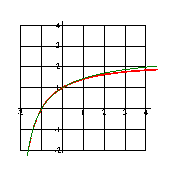
\includegraphics{cauchi/fig01a}} %b=sqrt(2) and b=exp(1/e)
\put(0,0){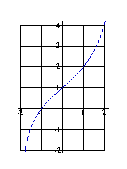
\includegraphics{cauchi/fig01b}} %b=2
\put(0,0){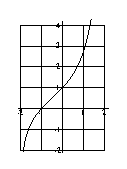
\includegraphics{cauchi/fig01c}} %b=e
\put(16,64.5){\sx{.25}{$\operatorname{sexp}_{b}(x)$}}
\put(33,65){\sx{.3}{$b\!=\!\rme$}}
\put(41.2,63){\sx{.25}{$b\!=\!2$}}
\put(52.3,42){\sx{.25}{$b\!=\!\exp(1/\rme)$}}
\put(53,36.4){\sx{.25}{$b\!=\!\sqrt{2}$}}
\put(65,20){\sx{.4}{$x$}}
\end{picture}}
\end{center}
\caption{Examples of tetrationals $\operatorname{sexp}_b(x)$ at base
$b\!=\!\rme$ (thick solid),
$b\!=\!2$ (dashed),
$b\!=\!\exp(1/\rme)$ (thin solid) and 
$b\!=\!\sqrt{2}$ (dotted) versus real $x$. 
%\iL{figreal}
\label{fig01abc}
}
\end{figure}

In generalization of the concept of a group acting on a set we could
say $\beta$ is an action of the semigroup $X$ on $D$ with
$\beta^1=f$. One only removes the demand of having inverses. 


END TODO

The above 3 concepts extended iteration, initialized superfunction and
Abel function are connected in the following way.
From each image-bijective TODO{whats that?} initialized superfunction $\sigma\colon
D\to(X\leftrightarrow D)$ of $f$ we obtain an image-bijective
initialized Abel function $\alpha = A(\sigma)\colon D\to(D\leftrightarrow
X)$ of $f$ by taking the inverse:
\begin{align*}
  A(\sigma)&:=\alpha & \alpha_u&=\sigma_u^{[-1]}.
\end{align*}
From each image-bijective initialized Abel function $\alpha\colon
D\to(D\leftrightarrow X)$ of
$f$ we obtain an $X$-iteration $B(\alpha)\colon X\to
(D\leftrightarrow D)$ of $f$
by
\begin{align*}
  B(\alpha)&:=\beta & \beta^t(z)&:=\alpha_u^{[-1]}(t+\alpha_u(z))
\end{align*}
which is independendant on $u$. It is also bijective in $t$ for fixed $z$. 

From each such $X$-iteration $\beta\colon X\to
(D\leftrightarrow D)$ of $f$ we
obtain an image-bijective initialized superfunction $\sigma\colon
D\to(X\leftrightarrow D)$
\begin{align*}
  S(\beta)&:=\sigma & \sigma_u(t)&:=\beta^t(u)
\end{align*}
for every $u\in D$. This last initialized superfunction is equal
to our initial initialized superfunction $\sigma$:
\begin{align*}
  (S B A(\sigma))_u(t) = \beta^t(u) = \alpha_u^{[-1]}(t+\alpha_u(u)) =
  \sigma_u(t), 
\end{align*}
We get the following further 3 identities
\begin{align*}
  S B A (\sigma)_u &= \sigma_u & A S B (\alpha)_u &= \alpha_u & B A S (\beta) &= \beta
\end{align*}
and see that these 3 concepts are interchangeable.

There is another related term ``iterative logarithm'' which was coined
by Jabotinsky \cite{Jabotinsky:Analytic} as it is similar to the behaviour of the natural
logarithm in several aspects (differently from the Abel function).

\begin{definition}[iterative logarithm, Julia
  equation]\label{def:julia_equation}
Let $f(D)\subseteq D$ be differentiable. A function $\lambda$ on $D$ that
satisfies the Julia equation
\begin{align}
  \lambda(f(x)) = f'(x)\cdot \lambda(x)\label{eq:julia_equation}
\end{align}
is called an {\em iterative logarithm} of $f$.
\end{definition}
You obtain this equation if you differentiate the Abel equation
\eqref{eq:abel_equation} and then set $\lambda(x)=1/\alpha_u'(x)$. 

Reversely if $\lambda$ satisfies the Julia equation then
$\gamma(z)=\int \frac{1}{\lambda(z)} dz$ satisfies
$\gamma(f(z))=\gamma(z)+c$ or equivalently
$\frac{1}{c}\gamma(f(z))=\frac{1}{c}\gamma(z)+1$.

For an iterative logarithm $\lambda$
\begin{align}
  \alpha_u(x)=\frac{1}{c}\int_u^x \frac{1}{ \lambda(\xi)} d\xi  \mt{where}
  c=\int_{f^{-1}(u)}^{u}
  \frac{1}{\lambda(\xi)} d\xi
\end{align}
is an initialized Abel function. The following left side is an
iterative logarithm if $\beta$ is an extended iteration of $f$, it
satisfies the relation on the right side.
%\label{eq:julia_beta} 
\begin{align}
  \lambda(x) &:= \left.\frac{\partial \beta^t(x)}{\partial t}\right|_{t=0}&
  \lambda(\beta^t(x))&=t\cdot \lambda(\beta(x)).
\end{align}
Compare the relations
\begin{align*}
  \left.\frac{\partial x^t}{\partial t}\right|_{t=0} &= \ln(x) & 
  \ln(b^t)&=t\cdot\ln(b)
\end{align*}
for the natural logarithm.

\subsection{Uniqueness} 

As the concepts extended iteration/superfunction/Abel function behave
similar like power/exponential/logarithm, we first repeat uniqueness
criterions for the latter concepts.

\begin{wellknown}\label{wk:exponential:real}
  For each $b>0$ there is exactly one real continuous function $f$ satisfying
  \begin{align*}
    f(1)&=b & f(s+t)&=f(s)f(t)
  \end{align*}
  and this solution is $f(x)=b^x$.
\end{wellknown}

Complex powers/exponentials lack the above uniqueness. Thatswhy we define the
following abbreviation:
\begin{definition}
  $b^{z;k} := \exp((\log(b)+2\pi i k)z)$ for $b\neq 0,w\in\C$,
  $k\in\Z$, where $\log$ is the standard logarithm determined by
  $-\pi<\Im(\log(z))\le \pi$. Omitting $;k$ means $k=0$:
  $b^z:=b^{z;0}$.
\end{definition}
We see that the complex function $f(z)=b^{z;k}$ satisfies the equations 
of knowledge \ref{wk:exponential:real} for each $k\in\Z$. 
The next proposition shows that these are indeed all holomorphic solutions.
\begin{wellknown}[$b^{w;k}$]\label{wk:exponential:holomorphic}
  Let $f$ be holomorphic in 0 satisfying $f(u+v)=f(u)f(v)$
  for all $u,v,u+v$ in some vicinity of 0. Then $f$ can be continued
  to an entire function. If $f(1)=b$ then $f(z)=b^{z;k}$ for some
  $k\in \Z$ and then $f'(0)=\log(b)+2\pi i k$.
\end{wellknown}


\section{${\mathfrak{R}}$egular Iteration}
Regular iteration is a well-investigated method due to the works of
Kœnigs \cite{MR1508749}, Schröder \cite{ref02.0042.02}, Lévy
\cite{levy:fonctions}, Szekeres
\cite{szekeres:regular}, Écalle \cite{Ecalle:InvariantsHolomorphes}, etc. 
Regular iteration with respect to a fixed point $z_0$ of $f$ is an
extended iteration $\beta$ of $f$ that is determined by being well-behaved at
$z_0$.
This means that $t\mapsto \beta^{t;k}$ being continuous
and each $z\mapsto \beta^{t;k}(z)$ being at least asymptotically
differentiable at $z_0$. 

In particular, with regular iterations one can evaluate the 
superexponential at base $b\le\exp{1/\rme}$. Four examples of the 
superexponentials for $b=\sqrt{2}$ are shown in figure \ref{figsqrt2}

%TODO only temporarily commented 
% %\newcommand \putE { \put(190,174) }
% \newcommand \putE { \put(215,174) }
% \newcommand \putL { \put(215,174) }
\begin{figure}
% \begin{center}
% \sx{.7}{\begin{picture}(300,210)\put(0,0){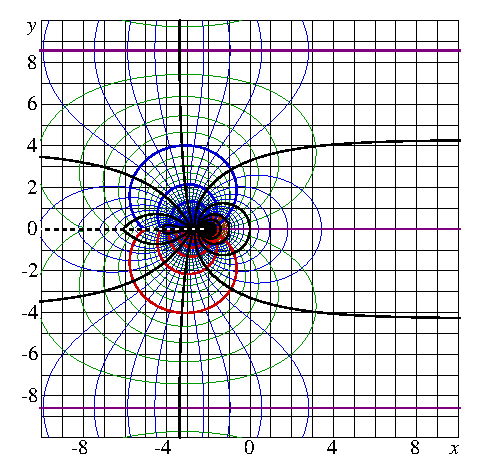
\includegraphics{cauchi/f21E}} 
% \putE{\sx{2}{$F_{2,1}(z)$}}
% \put(-24,194){\sx{1.2}{$q\!=\!0$}}
% \put(214,194){\sx{1.2}{$q\!=\!0$}}
% \put(214,151){\sx{1.2}{$p\!=\!2$}}
% \put(214,108){\sx{1.2}{$q\!=\!0$}}
% \put(214, 66){\sx{1.2}{$p\!=\!2$}}
% \put(-24, 21){\sx{1.2}{$q\!=\!0$}}
% \put(214, 21){\sx{1.2}{$q\!=\!0$}}
% \put(-21,108){\sx{1.2}{\bf cut}}
% \put(-24,144){\sx{1.2}{$p\!=\!4$}}
% \put(-24, 72){\sx{1.2}{$p\!=\!4$}}
% \put( 71,212){\sx{1.2}{$p\!=\!3$}}
% \put(131,212){\sx{1.2}{$p\!=\!2.2$}}
% \put(143,135){\sx{1.2}{$q\!=\!0.2$}}
% \put(147,119){\sx{1.2}{$p\!=\!1.8$}}
% \put(143, 77){\sx{1.2}{$q\!=\!-0.2$}}
% \put(141, 37){\sx{1.2}{$p\!=\!2.2$}}
% \end{picture}}
% \sx{.7}{\begin{picture}(240,210)\put(0,0){\ing{cauchi/f21L}} 
% \putL{\sx{2}{$F_{2,1}^{-1}(z)$}}
% \put( 24,198){\sx{1.2}{$Q\!=\!0$}}
% \put( 24,153){\sx{1.2}{$P\!=\!-2$}}
% \put( 24,108){\sx{1.2}{$Q\!=\!0$}}
% \put( 24, 60){\sx{1.2}{$P\!=\!-2$}}
% \put( 24, 16){\sx{1.2}{$Q\!=\!0$}}
% \put( 50, 29){\sx{1.1}{$P\!=\!-2.2$}}
% \put(137, 25){\sx{1.1}{$P\!=\!-2.8$}}
% \put( 50,180){\sx{1.1}{$P\!=\!-2.2$}}
% \put( 50,134){\sx{1.1}{$Q\!=\!0.2$}}
% \put( 43, 94){\sx{1.1}{$P\!=\!-1.8$}}
% \put( 44, 80){\sx{1.1}{$Q\!=\!-0.2$}}
% \put(210,108){\sx{1.2}{\bf cut}}
% \put(213, 49){\sx{1.0}{$Q\!=\!0$}}
% \put(214, 40){\sx{1.0}{$P\!=\!-3$}}
% \put(214, 31){\sx{1.0}{$P\!=\!-3$}}
% \put(214, 22){\sx{1.0}{$P\!=\!-3$}}
% \put(214, 14){\sx{1.0}{$P\!=\!-3$}}
% \end{picture}}
% \\
% \sx{.7}{\begin{picture}(300,220)\put(0,0){\ing{cauchi/f23E}}
% \putE{\sx{2}{$F_{2,3}(z)$}}
% \put(-22,194){\sx{1.2}{\bf cut}}
% \put(214,194){\sx{1.2}{$Q\!=\!0$}}
% \put(-24,157){\sx{1.2}{$P\!=\!4$}}
% \put(214,150){\sx{1.2}{$P\!=\!2$}}
% \put(173,141){\sx{1.1}{$Q\!=\!-0.2$}}
% \put(175,121){\sx{1.1}{$P\!=\!2.2$}}
% \put( 25,121){\sx{1.1}{$P\!=\!3.8$}}
% \put( 25, 71){\sx{1.1}{$Q\!=\!0.2$}}
% \put(175, 79){\sx{1.1}{$Q\!=\!0.2$}}
% \put(177, 31){\sx{1.1}{$P\!=\!1.8$}}
% \put(-24,107){\sx{1.2}{$Q\!=\!0$}}
% \put(214,107){\sx{1.2}{$Q\!=\!0$}}
% \put(214, 66){\sx{1.2}{$P\!=\!2$}}
% \put(-24, 57){\sx{1.2}{$P\!=\!4$}}
% \put(-22, 21){\sx{1.2}{\bf cut}}
% \put(214, 21){\sx{1.2}{$Q\!=\!0$}}
% \end{picture}}
% \sx{.7}{\begin{picture}(240,220)
% \put(0,0){\ing{cauchi/exc2cuts}}
% \put(0,0){\ing{cauchi/f23Lo}}
% \putL{\sx{2}{$F_{2,3}^{-1}(z)$}}
% %\put( 19,198){\sx{1.1}{\bf Q\!=\!-8.55}}
% \put( 19,206){\sx{1.1}{$Q\!=\!8.55$}}
% \put( 19, 26){\sx{1.1}{$Q\!=\!8.55$}}
% \put( 19,190){\sx{1.1}{$Q\!=\!-8.55$}}
% \put( 38,165){\sx{1.1}{$Q\!=\!-8.5$}}
% \put( 60, 52){\sx{1.1}{$Q\!=\!8.4$}}
% \put( 48, 38){\sx{1.1}{$Q\!=\!8.5$}}
% \put( -1,118){\sx{1.1}{$P\!=\!1.4$}}
% \put( -1,100){\sx{1.1}{$P\!=\!1.4$}}
% \put( 34,108){\sx{1.1}{\bf cut}}
% \put(214,108){\sx{1.1}{\bf cut}}
% \put(214, 46){\sx{1.1}{\bf cut}}
% \put(214, 35){\sx{1.1}{\bf cut}}
% \put(214, 25){\sx{1.1}{\bf cut}}
% \put(214, 18){\sx{1.1}{\bf cut}}
% \put(214, 10){\sx{1.1}{\bf cut}}
% \end{picture}}\\
% \sx{.7}{\begin{picture}(300,220)\put(0,0){\ing{cauchi/f43E}} 
% \putE{\sx{2}{$F_{4,3}(z)$}}
% \put(-24,204){\sx{1.2}{$Q\!=\!0$}}
% \put(200,204){\sx{1.2}{$\infty$}}
% \put(-24,157){\sx{1.2}{$P\!=\!4$}}
% \put(214,152){\sx{1.2}{$P\!=\!2$}}
% \put(-24,107){\sx{1.2}{$Q\!=\!0$}}
% \put(214,107){\sx{1.2}{$Q\!=\!0$}}
% \put(214, 64){\sx{1.2}{$P\!=\!2$}}
% \put(-24, 57){\sx{1.2}{$P\!=\!4$}}
% \put(-24, 11){\sx{1.2}{$Q\!=\!0$}}
% \put(200, 11){\sx{1.2}{$\infty$}}
% %\put( 15,107){\sx{1.2}{$Q\!=\!0$}}
% %\put(189,107){\sx{1.2}{$Q\!=\!0$}
% \put(175,141){\sx{1.1}{$Q\!=\!0.2$}}
% \put(175,121){\sx{1.1}{$P\!=\!2.2$}}
% \put( 25,121){\sx{1.1}{$P\!=\!3.8$}}
% \put( 25, 88){\sx{1.1}{$P\!=\!3.8$}}
% \put(173, 79){\sx{1.1}{$Q\!=\!-0.2$}}
% \put(177, 31){\sx{1.1}{$Q\!=\!1.8$}}
% \end{picture}}
% \sx{.7}{\begin{picture}(240,220)\put(0,0){\ing{cauchi/f43L}} 
% \putL{\sx{2}{$F_{4,3}^{-1}(z)$}}
% \put(93,193){\sx{1.2}{$P\!=\!1$}}
% \put(93, 18){\sx{1.2}{$P\!=\!1$}}
% \put(213,146){\sx{1.3}{$P\!=\!0$}}
% \put( 33,127){\sx{1.1}{$Q\!=\!-8.6$}}
% \put( 37, 86){\sx{1.1}{$Q\!=\!8.6$}}
% \put( 19,107){\sx{1.5}{\bf cut}}
% \put(215,108){\sx{1.4}{\bf cut}}
% \put(213, 72){\sx{1.3}{$P\!=\!0$}}
% \put(210, 40){\sx{1.3}{$Q\!=\!9$}}
% \put(212, 22){\sx{1.3}{$Q\!=\!0.4$}}
% \end{picture}}
% \\
% \sx{.7}{\begin{picture}(300,220) \put(0,0){\ing{cauchi/f45E}} 
% \putE{\sx{2}{$F_{4,5}(z)$}}
% \put( 54,194){\sx{1.1}{$P\!=\!3.8$}}
% \put(-28,204){\sx{1.3}{$Q\!=\!0$}}
% \put(216,204){\sx{1.3}{$Q\!=\!0$}}
% \put(215,156){\sx{1.3}{$P\!=\!2$}}
% \put(204,130){\sx{1.2}{$P\!=\!1.8$}}
% \put(211,120){\sx{1.2}{$Q\!=\!0$}}
% \put( 18,108){\sx{1.3}{$Q\!=\!0$}}
% %\put(216,108){\sx{1.3}{$Q\!=\!0$}}
% \put(206,108){\sx{1.3}{$\infty$}}
% \put(216, 59){\sx{1.3}{$P\!=\!2$}}
% \put(206,144){\sx{1.2}{$Q\!=\!0.2$}}
% \put(204, 45){\sx{1.2}{$Q\!=\!-0.2$}}
% \put(-28, 10){\sx{1.3}{$Q\!=\!0$}}
% \put(216, 10){\sx{1.3}{$Q\!=\!0$}}
% \put(-28,154){\sx{1.3}{$P\!=\!4$}}
% \put(-28, 61){\sx{1.3}{$P\!=\!4$}}
% %\put(121,216){$p\!=\!3$}
% \end{picture}}
% \sx{.7}{\begin{picture}(240,220)\put(0,0){\ing{cauchi/f45L}} 
% \putL{\sx{2}{$F_{4,5}^{-1}(z)$}}
% \put( 96,196){\sx{1.2}{$P\!=\!4$}}
% \put( 94, 18){\sx{1.2}{$P\!=\!4$}}
% \put(215,144){\sx{1.4}{$P\!=\!3$}}
% \put(215,108){\sx{1.4}{$Q\!=\!0$}}
% \put(215, 72){\sx{1.4}{$P\!=\!3$}}
% \put( 19,107){\sx{1.6}{\bf cut}}
% \put( 33,129){\sx{1.2}{$Q\!=\!1$}}
% \put( 33, 85){\sx{1.2}{$Q\!=\!-1$}}
% \end{picture}}
% \end{center}
% \caption{Functions
% $f\!=\!F_{2,1}(z)~$,
% $f\!=\!F_{2,3}(z)~$,
% $f\!=\!F_{4,3}(z)~$,
% $f\!=\!F_{4,4}(z)~$, left, and their inverse functions, right, in the 
% $z\!=\!x\!+\!\rmi y$ plane.
% Levels
% $\Re(f)\!=\!P\!=$const and levels
% $\Im(f)\!=\!Q\!=$const are shown with thick lines for integer values 
% of $P$ and $Q$.
  \label{figsqrt2}
% \iL{figq2F}}
\end{figure}


For real functions $f$ one presumes $f'(z_0)>0$ and distinguishes the
parabolic case $f'(z_0)=1$ from the other cases. (Complex functions
are called parabolic at $z_0$ if $f'(z_0)$ is a root of unity.)

\newcommand{\pso}{\mathfrak{P}_0}
We start this section with regular iteration of formal
powerseries with fixed point at 0, i.e.\ powerseries of the form
$f(z)=\sum_{n=1}^\infty f_n z^n$. We denote the set of these
powerseries with $\pso$. Later we consider the convergence
radius of these powerseries and present equivalent limit formulas.

\subsection{Formal Powerseries}
{\em Formal} powerseries mimic the behaviour of powerseries
developments of functions at 0, but have no need to converge. 
So for example $f(x)=x+2^2x^2+3^3x^3+\dots$ is a valid formal
powerseries though it does not converge for any $x$.

For a formal powerseries $f$ we usually denote the coefficient of
$x^n$ by $f_{:n}$. The formal powerseries $f$ is completely determined by
this sequence of its coefficients. So in this subsection we 
recall the formulas for the coefficients of the basic operations on
powerseries, particularly obtaining a formula for composition.


We start with the well-known formulas for addition and
multiplication.
\begin{align}
  \left(\sum_{n=0}^\infty f_{:n} x^n\right) + \left(\sum_{n=0}^\infty
    g_n x^n\right)&=\sum_{n=0}^\infty (f_{:n}+g_{:n})x^n & (f+g)_n &=
  f_{:n} + g_{:n}\label{eq:powerseries:addition}\\
  \left(\sum_{n_1=0}^\infty f_{:n_1} x^{n_1}\right)
  \left(\sum_{n_2=0}^\infty g_{:n_2} x^{n_2}\right)&=
  \sum_{n,m=0}^\infty f_{:n_1} g_{:n_2} x^{n_1+n_2} &
(fg)_n &= \sum_{n_1+n_2=n} f_{:n_1} g_{:n_2}\label{eq:powerseries:multiplication}
\end{align}
Division by $f$ can be performed when $f_{:0}\neq 0$. We can derive the
recursive formula of $g=1/f$ by solving $fg=1$ for $g$:
\begin{align*}
  g_{:0} &= \frac{1}{f_{:0}} & g_{:n} &=
  -\frac{1}{f_{:0}}\sum_{k=0}^{n-1} f_{:n-k}
  g_{:k},\quad n\ge 1
\end{align*}
When taking powers, note that ${f^m}_{:n}$ means the $n$-th coefficient of
the $m$-th power of $f$, while ${f_{:n}}^m$ means the $m$-th power of the
$n$-th coefficient of $f$. Deriving from
\eqref{eq:powerseries:multiplication} we get
\begin{align}\label{eq:powerseries:power}
  {f^m}_{:n} = \sum_{n_1+\dots+n_m=n} f_{:n_1}\dotsm f_{:n_m} =
  \sum_{\substack{m_1+2m_2+\dots+nm_n = n\\m_0+\dots+m_n=m}}
    \frac{m!}{m_0!\dotsm m_n!}{f_{:0}}^{m_0}\dotsm {f_{:n}}^{m_n}
\end{align}
This enables a formula for composition
\begin{align*}
  f(g(x))&=\sum_{m=0}^\infty f_{:m} g(x)^m &
  (f\circ g)_{:n} &= \sum_{m=0}^\infty f_{:m} {g^m}_n
\end{align*}
which may however problematic as we dont know about the convergence of
each coefficient. A minor constraint on $g$ however makes the
coefficients finite expressions.

If $g_{:0}=0$ then ${g^m}_{:n} = 0$ for $n<m$. Hence
\begin{align}\label{eq:powerseries:composition}
  (f\circ g)_{:n} &= \sum_{m=0}^n f_{:m} {g^m}_{:n}, \quad g_0=0.
\end{align}


\begin{definition}[$\pso$]
  That's why we introduce the symbol $\pso$ for the set of formal powerseries $f$ with $f_0=0$.
\end{definition}
It is closed under addition, multiplication and composition.

\subsubsection{Non-Parabolic regular iteration of formal powerseries}
\label{sec:Non-parabolic powerseries}

We first notice that $(f\circ g)_1 = f_1g_1$ 

\newcommand{\regitn}[1]{{#1}^{\mathfrak{R}:}}
\newcommand{\regitOn}[2]{{#1}^{\mathfrak{R}#2:}}
\newcommand{\regitO}[2]{{#1}^{\mathfrak{R}:#2}}
\newcommand{\regit}[3]{{#1}^{\mathfrak{R}#2:#3}}
\begin{wellknown}[regular iteration on non-parabolic powerseries]
  \label{wk:iteration:powerseries:non-parabolic:real}
  Let $P$ be the set of formal powerseries $f\in\pso$ with $0<{f_1}$
  and $f_1\neq 1$. Then there exists exactly one $\R$-iteration $\beta$
  of $f$ such that $\beta^t \in P$ for each $t\in\C$ and such
  that $t\mapsto {\beta^t}_1$ is continuous. It is
  called the {\em regular iteration} of $f$ and written as
  $\beta=\regitn{f}$. 
\end{wellknown}
\begin{proof}TODO.
Uniqueness: consider the function $h(t)={\beta^t}_1$. Then by
definition \ref{def:extended_iteration} of the extended iteration:
$h(1)=f_1$ and $h(s+t)=(\beta^s\circ \beta^t)_1= h(s)\cdot h(t)$. By
continuity $h(t)={f_1}^t$.
\end{proof}

The regular iteration of $f$ is recursively given by the
following formula where $g:=\regitO{f}{t}$: 
\begin{align}\label{eq:non-parabolic:powerseries}
  g_1 &= {f_1}^t & g_n = \frac{1}{{f_1}^n - f_1} \left(
    f_n {g_1}^n - g_1 f_n + \sum_{m=2}^{n-1} f_m {g^m}_n - g_m
    {f^m}_n
  \right)
.\end{align}


This proposition can be generalized in the spirit of knowledge
\ref{wk:exponential:holomorphic} 
\begin{proposition}[Complex regular iteration on non-parabolic powerseries]
  \label{wk:iteration:powerseries:non-parabolic:complex}
  Let $P$ be the set of formal powerseries $f\in\pso$ with
  ${f_1}^n\neq f_1$ for all integer $n\ge 2$. If
  $\beta$ is an $\C$-iteration of $f$ such that
  $\beta^w \in P$ for each $w\in\C$ and such that $w\mapsto
  {\beta^w}_1$ is holomorphic in 0 then there exists a $k\in\Z$ such
  that ${\beta^w}_1 = {f_1}^{w;k}$.

  For each $k\in\Z$ there exists a unique $\C$-iteration $\beta$
  such that ${\beta^{w;k}}_1={f_1}^{w;k}$ which is
  called the {\em regular iteration} of $f$. Each ${\beta^{w;k}}_n$ is a
  polynomial in $f_1^{w;k}$.
\end{proposition}
\begin{proof}
  TODO
  $\beta$ is recursively given by \eqref{eq:non-parabolic:powerseries} when
  replacing ${f_1}^t$ by ${f_1}^{w;k}$.
\end{proof}

\begin{wellknown}[principal Schröder powerseries]
  Let $f\in \pso$ be a formal powerseries with ${f_1}^n\neq f_1$
  for all postive integers $n$, then
  there exists exactly one formal powerseries $\chi$ with
  $\chi_0=0$ and $\chi_1=1$ such that $\chi\circ f = f_1\cdot\chi$. 
  It is called the {\em principal Schröder powerseries} of $f$.
\end{wellknown}
The principial Schröder powerseries is recursively given by:
\begin{align}
  \chi_1 &= 1 & \chi_n = \frac{1}{f_1-{f_1}^n}\sum_{m=1}^{n-1}
  \chi_m {f^m}_n.
\end{align}
The inverse $\chi^{[-1]}$ of the principal Schröder powerseries is recursively given by:
\begin{align}
  {\chi^{[-1]}}_1 & = 1 & {\chi^{[-1]}}_n &= \frac{1}{{f_1}^n - f_1}\sum_{m=1}^{n-1}
  f_m {\left(\chi^{[-1]}\right)^m}_n
\end{align}

\begin{wellknown}
  Let $f\in \pso$, let $\beta$ be the regular iteration of $f$
  and let $\chi$ be the principal Schröder powerseries of $f$. Then
  \begin{align}
    \beta^{w;k}(u) &= \chi^{[-1]}({f_1}^{w;k} \cdot \chi(u)) = z\\
    \alpha_u(z) &= \log_{f_1;k}\frac{\chi(z)}{\chi(u)} = w
  \end{align}
\end{wellknown}

\begin{align}
  \label{eq:julia_npar}
  \lambda_0&=0,\quad \lambda_1=1\\
  \lambda_n&= \frac{1}{{f_1}^n - f_1} \sum_{m=1}^{n-1} \lambda_m
  \left( (n-m+1)f_{n-m+1}  - {f^m}_n \right)
\end{align}

\subsubsection{Parabolic iteration of powerseries}
\label{sec:Parabolic powerseries}
\newcommand{\psoi}{\mathfrak{P}_{01}}
\newcommand{\psoiN}[1]{\mathfrak{P}_{01,#1}}
\begin{definition}
  Let $\psoiN{N}$ be the set of formal powerseries $f$ with $f_N\neq
  0$ and $f_n = \id_n$ for $n<N$. Let $\psoi$ be the union of all
  $\psoiN{N}$, $N\ge 2$.
\end{definition}
We first notice that $(f\circ g)_N=f_N+g_N$ for $f,g\in\psoiN{N}$.

Let us now consider the parabolic case:
\begin{wellknown}[regular iteration on parabolic
  powerseries]\label{wk:iteration:powerseries:parabolic}
  For each $f\in \psoi$ there exists a unique $\C$-iteration $\beta$ 
  of $f$ such that $\beta^t \in \psoi$ for each $t\in\C$ and such
  that each $t\mapsto {\beta^t}_n$ is continuous. The functions
  $t\mapsto {\beta^t}_n$ are polynomials. $\beta$ is
  called the {\em regular iteration} of $f$. It is given by
  \begin{align}
    \label{eq:parabolic_regular_iteration}
    {\beta^t}_1&=1 & {\beta^t}_n&=\sum_{m=0}^{n-1} \binom{t}{m} \sum_{k=0}^m \binom{m}{k} (-1)^{m-k}
    {f^{[k]}}_{n}
  \end{align}
\end{wellknown}
TODO reference to Jabotinsky

A direct recursive formula for the coefficients can be given but it is
too cumbersome to derive it at this place. Instead we refer to the
formula by Jabotinsky TODO.

TODO
Abel function as the Inverse of the superfunction $z_0+\chi^{-1}(b^z)$ is $\log_b(\chi(z-z_0))$ (non-parabolic).
\subsubsection{The regular Abel function via the Julia equation and iterative logarithm}
The regular Abel function has a singularity at the fixed point of
development, so we can not give a pure powerseries development as  for the extended iteration
of $f$. But we can obtain something similar.

By differentiating the Abel equation we get
$\alpha'(f(x))f'(x)=\alpha'(x)$. Though $\alpha'$ can not be a
powerseries when $\alpha$ isn't, it appears that
$j(x)=1/\alpha'(x)$ can be presented as a powerseries.

It satisfies the Julia equation, see \eqref{eq:julia_equation}.
\newcommand{\logit}{\operatorname{logit}}
\begin{wellknown}[iterative logarithm powerseries]
  Let $f\in \pso$ such that either $f_1=1$ or $f_1$ not being a
  primitive root of unity, let $(f-\id)_n=0$ for $n<N$ and
  $(f-\id)_N\neq 0$ 
  then there is exactly one solution
  $\lambda\in\pso$ with $\lambda_n=0$ for $n<N$ and $\lambda_N=1$
  that satisfies the Julia equation \eqref{eq:julia_equation}.
  It is called the {\em iterative
    logarithm powerseries} of $f$ and we write $\lambda=\logit[f]$. 
  In the parabolic case $N\ge 2$ it is given by
  \begin{gather}
    \lambda_{n} = \sum_{m=0}^{n-1} \frac{s(m,1)}{m!}\sum_{k=0}^m
    \binom{m}{k} (-1)^{m-k} {f^{[k]}}_n
  \end{gather}
  where $s(m,k)$ is the stirling number of the first kind and in the
  non-parabolic case $N=1$ it is recursively given by
  \begin{align}
    \lambda_1 &= 1 &
    \lambda_n &= \frac{1}{f_1^n-f_1}\sum_{k=1}^{n-1}
    ((n+1-k)f_{n+1-k}-{f^k}_n) \lambda_{k},\quad n\ge 2.
  \end{align}
\end{wellknown}

So generally the iterative logarithm powerseries is of the form:
\begin{align}
  \label{eq:julia_form}
  \lambda(z) = \sum_{n=N}^\infty \lambda_n z^n 
  = z^N\sum_{n=0}^\infty \lambda_{n+N} z^n,\quad \lambda_N\neq 0
\end{align}
Hence its reciprocal can be given as
\begin{align}
  \frac{1}{\lambda(z)} = z^{-N}\frac{1}{\sum_{n=0}^\infty
    \lambda_{n+N} z^n} = \sum_{n=-N}^\infty h_n z^n
\end{align}
and integrated
\begin{align}\label{eq:Abel_Julia}
\int \frac{1}{\lambda(z)} dz = 
\underbrace{\sum_{n=-N}^{-2} h_n\frac{z^{n+1}}{n+1} + h_{-1}
  \log(z)}_{\tilde{\alpha}(z)} + \sum_{n=0}^\infty h_n\frac{z^{n+1}}{n+1} .
\end{align}

Once we know this representation we can directly compute the
coefficients in $\alpha_{-N+1}z^{-N+1} + \dotsb +
\alpha_{-1}z^{-1} + \alpha_\ast \log(z)$.


\begin{proposition}
  Let $\lambda$ be the iterative logarithm powerseries of
  $f\in\pso$. Let 
  \begin{align*}
    \gamma(z)&=\int \frac{1}{\lambda(z)} dz\\
    \alpha_u(z)&=\frac{\gamma(z)-\gamma(u)}{c} &
    c&=\begin{cases}\log(f_1)& N=1\\f_N & N\ge 2\end{cases}
  \end{align*}
  then $\alpha_u$ is the regular Abel function of $f$.
\end{proposition}

TODO
In the non-parabolic case $N=1$ we obtain
$c={\gamma(f(u))-\gamma(u)}={\log(f_1)}$ and in the
parabolic case we obtain $c=f_N$.


TODO search better place for this proposition, which is needed in the
application to exponentials
\begin{proposition}\label{prop:regular_conjugate_iterate}
  $\regitO{(g^{[-1]}\circ f\circ g)}{w}=g^{[-1]}\circ \regitO{f}{w} \circ
  g$ for any $f,g\in\pso$ such that the equation is defined.
\end{proposition}

\subsection{Limit Formulas}

From the last formula \eqref{eq:Abel_Julia} we can already derive a
limit formula. Considering $\alpha(f^{[n]}(x))=n+\alpha(x)$ and
$\alpha(z)-\tilde{\alpha}(z)\to 0$ for $z\to 0$ we obtain for
$0<|f_1|<1$ (attractive fixed point at 0)
\begin{align}\label{eq:Ecalle}
  \alpha(x)=\lim_{n\to\infty} \tilde{\alpha}(f^{[n]}(z)) - n
\end{align}

\subsubsection{Non-Parabolic}
\label{sec:Non-parabolic limit}
\begin{proposition}[Principal Schr\"oder function]
  Let $f\in \pso$ with $0<\abs{f_1}<1$ have positive convergence radius
  then the principal Schr\"oder powerseries $\chi$ of $f$ has positive
  convergence radius too and is equal to the limit
  \begin{align*}
    \chi(x) &= \lim_{n\to\infty} \frac{f^{[n]}(x)}{{f_1}^n} 
  \end{align*}
  for each $x$ in the basin of attraction of $f$ at the fixed point 0.
  \begin{align*}
    \chi^{[-1]}(x) &= \lim_{n\to\infty} f^{[-n]}\left({f_1}^n\cdot
      x\right) 
  \end{align*}
  ($f^{[-1]}$ is the local inverse of $f$ at 0.)
\end{proposition}

\begin{proposition}[Regular iteration]\label{schroeder_radius}
  Let $f\in\pso$ with $0<\abs{f_1}<1$ have positive convergence radius
  then each regular iterate $\beta^t$ of $f$ has positive radius of
  convergence and is equal to the limit
  \begin{align*}
    \beta^{t;k}(u)&=\lim_{n\to\infty} f^{[-n]}\left({f_1}^{t;k}\cdot f^{[n]}(u)\right)=v\\
    \chi_u(v)&=\lim_{n\to\infty}
    \frac{f^{[n]}(v)}{f^{[n]}(u)}={f_1}^{t;k}
  \end{align*}
\end{proposition}

\subsubsection{Parabolic}
\label{sec:Parabolic limit}
TODO Powerseries has usually 0 convergence radius, but asymptotic
powerseries. How to compute the function with non-converging
powerseries (Julia-equation). Jabotinksy (better after matrices).

\begin{align}\label{eq:Levy}
  \beta^t(u)&= \lim_{n\to\infty}f^{[-n]}((1-t)\cdot f^{[n]}(u)+t\cdot f^{[n+1]}(u))=v\\
  \alpha_u(v)&=\lim_{n\to\infty}\frac{f^{[n]}(v) -
    f^{[n]}(u)}{f^{[n+1]}(u)-f^{[n]}(u)}=t
\end{align}
\begin{align}\label{eq:Levy2}
  \alpha(v)&=\lim_{n\to\infty}\frac{f^{[n]}(v)-f^{[n]}(u)}{f_N
    (f^{[n]}(u))^N},\quad N\ge 2
\end{align}
where $N$ is the smallest number where $f$ deviates from $\id$.

The powerseries development of the Abel function can be used despite
non-convergence in the following way:
$\tilde{\alpha}=\int \frac{dz}{\lambda(z)}$
\begin{align}
  \alpha(z)=\lim_{n\to\infty} \tilde{\alpha}(f^{[n]}(z))-n
\end{align}

%TODO: regular iteration is invariant to compositional conjugation
%(that keeps the fixed point)

\subsubsection{Non-Zero Fixed Point}
The previous formulas all assume that the fixed point is at 0. If we
have a function $f$ with fixed point at $z_0$ then we just consider
the by a translation conjugated function $h(x)=f(x+z_0)-z_0$. This
function has the fixed point at 0, can be iterated there and it then
will be conjugated back.

\begin{definition}
  Let $f$ be a function with fixed point at $z_0$, let
  $h(z):=f(z+z_0)-z_0$,
  we call 
  \begin{align}
    \regit{f}{z_0}{w}(z)=\regitO{h}{w}(z-z_0)+z_0 
  \end{align}
  the regular iteration of $f$ at $z_0$.
\end{definition}
If we set $\tau_{z_0}(z):=z+z_0$ then we can write $h=\tau_{z_0}^{[-1]}\circ f
\circ \tau_{z_0}$ and the above formula as 
\begin{align}
	\regit{f}{z_0}{w}=\tau_{z_0}\circ \regitO{h}{w}\circ \tau_{z_0}^{[-1]}
\end{align}

Accordingly we rewrite the limit formulas for this general case,
noticing that $(g^{[-1]}\circ f\circ g)^{[n]}=g^{[-1]}\circ f^{[n]}
\circ g$:

\begin{proposition}\label{hyperbolic_iteration}
Let $f$ be holomorphic at $z_0$ and $\lambda:=f'(z_0)$ with
$0<|\lambda|<1$, the regular iteration $\beta$ and the regular
Schröder functions $\chi_z$ of $f$ at $z_0$ are given by the limit
formulas
\begin{align}
  \beta^{w;k}(z)&=\lim_{n\to\infty}
  f^{[-n]}\left((1-\lambda^{w;k})\cdot z_0+\lambda^{w;k}\cdot f^{[n]}(z)\right)=v\\
  \chi_z(v)&=\lim_{n\to\infty}
  \frac{f^{[n]}(v)-z_0}{f^{[n]}(z)-z_0}=\lambda^{w;k}
.\end{align}
\end{proposition}

\begin{proposition}[Lévy formula, parabolic iteration]\label{prop:Levy2}
  Let $f$ be holomorphic at $z_0$ and $f'(z_0)=1$, the regular
  iteration $\beta$ and the regular initialized Abel function $\alpha$ of $f$ at
  $z_0$ are given by the (from $z_0$ independent) limit formulas
  \begin{align}
    \beta^w(z)&= \lim_{n\to\infty}f^{[-n]}((1-w)\cdot f^{[n]}(z)+w\cdot f^{[n+1]}(z))=v\\
    \alpha_z(v)&=\lim_{n\to\infty}\frac{f^{[n]}(v) - f^{[n]}(z)}{f^{[n+1]}(z)-f^{[n]}(z)}=w
  .\end{align}
\end{proposition}

Be careful that the above limit may also exist for functions with
$f'(z_0)\neq 1$ where it will not give the regular itertion/Abel
function but under the conditions of proposition \ref{hyperbolic_iteration}:
\begin{align}
  \lim_{n\to\infty}
  \frac{f^{[n]}(v)-f^{[n]}(z)}{f^{[n+1]}(z)-f^{[n]}(z)}=\left(w+\frac{2\pi i
    k}{\log \lambda}\right)\frac{1-\lambda^{w;k}}{1-\lambda}
\end{align}

\subsection{Application to Exponentials}
\subsubsection{formal powerseries iterates}
We conjugate $f(x)=b^x$ to 
\begin{align*}
  h_1(x)&=f(x+b^-)-b^-=b^-(\rme^{\ln(b)x}-1)=\frac{1}{\ln b} h(x\ln b)\\
  h(x)&=\ln(b)b^-(e^x-1)=\underbrace{\ln(b^-)}_{f'(b^-)=:a}(e^x-1)
\end{align*}
which has the powerseries development 
\begin{align*}
  h_0 &= 0 & h_n &= \frac{a}{n!}, \quad n>0
\end{align*}

Regular $\C$-iteration:
\begin{align*}
\regitO{h}{t}(z) &= sz+\frac{\frac{1}{2} s^{2} - \frac{1}{2} s}{a -
  1}z^2+\frac{\frac{1}{6} a s^{3} - \frac{1}{2} a s^{2} + \frac{1}{3}
  s^{3} + \frac{1}{3} a s - \frac{1}{2} s^{2} + \frac{1}{6} s}{a^{3} -
  a^{2} - a + 1}z^3+\dotsb,\quad s=a^t\\
\regit{f}{b^-}{t}(z) &= b^-+\frac{1}{\ln b}\regitO{h}{t}((z-b^-)\ln
b)
%\\ &= b^- + s(z-b^-)+\frac{\frac{1}{2} s^{2} - \frac{1}{2} s}{a - 1}\ln(b) (z-b^-)^2+\frac{\frac{1}{6} a s^{3} - \frac{1}{2} a s^{2} + \frac{1}{3} s^{3} + \frac{1}{3} a s - \frac{1}{2} s^{2} + \frac{1}{6} s}{a^{3} - a^{2} - a + 1}\ln(b)^2(z-b^-)^3+\dotsb
\end{align*}

$\alpha$ obtained through the Schröder equation:
\begin{align*}
\chi_h(z)&=z+\frac{\frac{1}{2}}{-a + 1}z^2+\frac{\frac{1}{3} a +
  \frac{1}{6}}{a^{3} - a^{2} - a + 1}z^3+\frac{-\frac{1}{4} a^{3} -
  \frac{5}{24} a^{2} - \frac{1}{4} a - \frac{1}{24}}{a^{6} - a^{5} -
  a^{4} + a^{2} + a - 1}z^4 + \dotsb\\
\alpha_{\mathfrak{R}}[h](z)&=\log_a(\chi(z))\\
\alpha_{\mathfrak{R}b^-}[f](z)&=\alpha_{\mathfrak{R}}[h]((z-b^-)\ln
b)=\log_a(\chi((z-b^-)\ln b))
\end{align*}

$\alpha$ obtained through the Julia equation:
\begin{align*}
\alpha_{\mathfrak{R}}[h](z)\ln a= \log(z)+\frac{\frac{1}{2}}{-a +
  1}z+\frac{\frac{5}{24} a + \frac{1}{24}}{a^{3} - a^{2} - a +
  1}z^2+\frac{\frac{1}{8} a^{3} + \frac{1}{24} a^{2} + \frac{1}{12}
  a}{-a^{6} + a^{5} + a^{4} - a^{2} - a +
  1}z^3 +\dotsb
\end{align*}

\begin{align*}
  \alpha_{\mathfrak{R}}[h](z) &= \lim_{n\to\infty} \log_a(h^{[n]}(z)) - n
  = \log_a\frac{h^{[n]}(z)}{a^n}
\end{align*}

TODO refer back to the particular methods
TODO refer to appendix for overview of fixpoints
\newcommand{\sfrt}{\operatorname{sr}}
\subsubsection{limit formulas}
To get the regular tetrational we apply this to $f(x)=b^x=\exp_b(x)$
at its lower fixed point $b^-=\sfrt^{[-1]}_+(b)$. The
derivative at the fixed point $b^-$ is $\lambda=\exp_b'(b^-)=\ln(b^-)$
by knowledge \ref{wk:fixedpoint:formula}.
\begin{definition}
  For $1<b\le \eta$ we define $\rsexp_b(x)$ to be the regular
  superfunction $\sigma_1$ of $z\mapsto b^z$ at its lower real fixed
  point $b^-$.
\end{definition}

\begin{align}
  b^-&=\exp(-W(-\ln b))=\frac{W(-\ln b)}{-\ln b}\\
  \rsexp_b(w)&=\lim_{n\to\infty}
  \log_b^{[n]}\left((1-(\ln b^-)^{w})\cdot b^-+(\ln b^-)^{w}\cdot \exp_b^{[n]}(1)\right)
\end{align}
\begin{align}
  \operatorname{rslog}_b(x)=\lim_{n\to\infty} \log_{\ln(b^-)} \frac{\exp_b^{[n]}(x)-b^-}{\exp_b^{[n]}(1)-b^-}
\end{align}  

The parabolic case occurs for $b=\rme^{1/\rme}$ and fixed point $\rme$. The Lévy formula
\eqref{eq:Levy2} converges much too slow to be applicable. 

Conjugating the fixed point $e$ of $f(x)=\rme^{x/\rme}$ to 0, we obtain:
\begin{align*}
  h_1(x)=f(x+\rme)-\rme=\rme^{(x+\rme)/\rme}-\rme=\rme(\rme^{x/\rme} -1)
\end{align*}
We can further simplify the conjugated function to
\begin{align*}
  h(x)=\rme^x-1, h_1(x)=\rme h(x/\rme)
\end{align*}
while knowing by proposition \ref{prop:regular_conjugate_iterate} that
$\regitO{h_1}{w}(z)=\rme\regitO{h}{w}(z/\rme)$ and of course
$\regit{f}{\rme}{w}(z)=\regitO{h_1}{w}(z-\rme)+\rme$, together:
\begin{align*}
  \regit{f}{\rme}{w}(z)=\rme\regitO{h}{w}\left(\frac{z}{\rme}-1\right)+\rme
\end{align*}

\begin{align*}
\lambda(x)=x^2-\frac{1}{6}x^3+\frac{1}{24}x^4-\frac{1}{90}x^5+\frac{11}{4320}x^6-\frac{1}{3360}x^7+\dots
\end{align*}
From this iterative logarithm one can get a description of the regular
Abel function by $\alpha = \frac{1}{f_2}\int \frac{1}{\lambda}$.
\begin{align*}
\alpha'(x)=\frac{1}{\lambda(x)}=x^{-2}+
\frac{1}{6}x^{-1}-\frac{1}{72}+\frac{1}{540}x+\frac{1}{5184}x^2-\frac{71}{217728}x^3+\dots
\end{align*}
If we integrate this and divide by $f_2=\frac{1}{2}$ to get $\alpha$ the term $x^{-1}$ becomes
$\ln(x)$ for $x>0$:
\begin{align}
\alpha(x)=\underbrace{-2x^{-1}+\frac{1}{3}\ln(x)}_{\tilde{\alpha}(x)}
-\frac{1}{36}x+ \frac{1}{540}x^2+
\frac{1}{7776}x^3 -\frac{71}{435456}x^4+
\dots
\end{align}

Instead we
get good results with Écalle's formula \eqref{eq:Ecalle}.
To use this formula we h
  

\section{${\mathfrak{M}}$atrix power iteration}
\label{sec:Matrix power}
The basic observation for this method is that the composition of
powerseries can be accomplished by the multiplication of certain
associated matrices, the so called Carleman matrices:

\newcommand{\carl}[1]{\operatorname{C}[#1]}
\newcommand{\Carl}[1]{\operatorname{C}\left[#1\right]}
\newcommand{\carlt}[2]{\operatorname{C_#2}[#1]}
\newcommand{\Carlt}[2]{\operatorname{C_#2}\left[#1\right]}
\begin{definition}
  Let $f$ be a formal powerseries. We define the Carleman matrix
  $\carl{f}$ as the infinite matrix that has as $m$-th row the
  coefficients of the powerseries $f^m$. The columns and rows here
  start at index 0, respectively. Formally:
  \begin{align}
    \carl{f}_{m,n} &= {f^m}_{:n}&& m,n\in \NZ
  \end{align}
\end{definition}

\begin{wellknown}
  For formal powerseries $f$ and $g$ with $g_0=0$ we have 
  $\carl{f\circ g}=\carl{f}\carl{g}$
\end{wellknown}
\begin{proof}
  Look at formula for powerseries composition
  \eqref{eq:powerseries:composition} and apply the formula for
  powerseries powers \eqref{eq:powerseries:power} while noticing that
  ${g^k}_i=0$ for $i<k$ because $g_0=0$: 
  \begin{align*}
    {(f\circ g)^m}_{:n} &= \sum_{n_1+\dots+n_m=n} \left(\sum_{k=0}^{n_1}
      {f}_{:k} {g^k}_{:n_1} \right)\dotsm \left(\sum_{k=0}^{n_m} {f}_{:k}
      {g^k}_{:n_m}\right)\\
      &= \sum_{k=0}^n \left(\sum_{k_1+\dots+k_m=k} f_{:k_1}\dotsm
        f_{:k_m}\right) {g^k}_{:n} = \sum_{k=0}^n {f^m}_{:k} {g^k}_{:n}
%\left(\sum_{n_1+\dots+n_k=n} g_{n_1}\dotsm g_{n_k}\right)
  \end{align*}
\end{proof}

%TODO: matrix power iteration is purely on formal powerseries no
%investigation of limit methods or of the convergence radius of the
%resulting powerseries (except in the case of regular iteration) is
%done yet.

\subsection{Holomorphic Functions on Matrices}
The most obvious way to apply a holomorphic function $f(z)=f_{:0} +
f_{:1} z + f_{:2} z^2 + \dots$ to a matrix $A$ is just by $f(A)=f_{:0} + f_{:1} A
+ f_{:2} A^2 + \dots$. However this approach does not always work: If the
eigenvalues of $A$ are not completely contained in the disk of
convergence then the above method will fail.

We start with simpler matrices of the form
\begin{align}\label{eq:matrix:simple}
  A = \begin{pmatrix}
    \lambda & a_{1,2} &\dots & a_{1,N-1} &a_{1,N}\\
    0 & \lambda & \dots & a_{2,N-1} & a_{2,N}\\
     &  & \vdots &\\
    0 & 0 & \dots & \lambda & a_{N-1,N} \\
    0 & 0 & \dots & 0 &\lambda
  \end{pmatrix}
\end{align}
because then the matrix $A-\lambda I$ is nilpotent, $(A-\lambda
I)^N= 0$. This means we do not need to take infinite sums:

\begin{sdef}
For matrices of the form \eqref{eq:matrix:simple} we define the
application of the holomorphic function $f$ with powerseries
development $f(z)=\sum_{n=0}^\infty f[z_0]_{:n} (z-z_0)^n$ at
$z_0$ as 
  \begin{align*}
    f(A):=\sum_{n=0}^{N-1} f[z_0]_{:n} (A-z_0 I)^n.
  \end{align*}
\end{sdef}

To make the application of the function invariant to matrix similarity
we extend the definition to arbitrary square matrices $A$ as follows.

\begin{sdef}
  Let $f$ be a holomorphic function on $D$ and let $A$ be $N\times N$ square
  matrix with eigenvalues $\lambda_i\in D$, $1\le i \le l$, which have multiplicities
  $\mu_i\ge 1$, $\mu_1+\dotsb+\mu_l=N$. Let $A=SJS^{-1}$ be the Jordan normal form of $A$ with
  $J=J_1\oplus\dotsb \oplus J_l$, where $J_i$ is the
  $\mu_i\times\mu_i$ Jordan block corresponding to $\lambda_i$ (having
  $\lambda_i$ on the diagonal and $1$ on the upper secondary
  diagonal if $\mu_i\ge 2$). We define
  \begin{align}
    f(A):=S\left( f(J_1)\oplus\dotsb\oplus f(J_l)\right) S^{-1}.
  \end{align}
  This definition is independent on the particular Jordan
  decomposition.
\end{sdef}
Indeed this definition is invariant under matrix similarity:
\begin{wellknown}
  Let $f$ be holomorphic on $D$ then 
  \begin{align}
    f(L^{-1}AL)=L^{-1}f(A)L
  \end{align}
  for any $N\times N$ square matrix $A$ that has all eigenvalues in $D$ and any
  invertible $N\times N$ matrix $L$. 
\end{wellknown}
Our definition coincides with direct application of the powerseries
to the matrix if it converges:
\begin{wellknown}\label{prop:matrixfunction:powerseries}
  Let $f$ be a holomorphic function on $D$ with powerseries expansion
  $f(z)=\sum_{n=0}^\infty f[z_0]_{:n} (z-z_0)^n$ at $z_0\in D$. Let $A$
  be a complex square matrix with all eigenvalues contained in the
  convergence disk of $f$ around $z_0$. Then
  \begin{align*}
    f(A)=\sum_{n=0}^\infty f[z_0]_{:n} (A-z_0 I)^n.
  \end{align*}
\end{wellknown}
Additionally the definition satsifies the following properties
\begin{wellknown}
  Let $f,g$ be holomorphic on $D$ then
  \begin{align}
    %(f+g)(A)&=f(A)+g(A)\\
    (fg)(A)&=f(A)g(A)\label{eq:matrix:function:multiplication}
  \end{align}
  for every square matrix $A$ that has all eigenvalues in $D$.
\end{wellknown}
For proofs of these propositions see e.g.\ \cite{horn:topics}.

With the previous establishments we can now easily define arbitrary
powers of a a square matrix. 

\begin{definition}[matrix power]
  Let $A$ be a square matrix having only non-zero eigenvalues, we define
  {\em the matrix power} by $A^{w;k}:=f_{w,k}(A)$ where $f_{w,k}(z):=z^{w;k}$.
\end{definition}
\begin{proposition}\label{prop:matrixpower:exponents}
  $A^{1;k}=A$ and $A^{v+w;k} = A^{v;k} A^{w;k}$ for all complex $v,w$ and integer $k$.
\end{proposition}
\begin{proof}
  Let $f_{w;k}(z)=z^{w;k}=\exp(({\log}(z)+2\pi i k)w)$ then
  $f_{v+w;k}(z)=z^{v+w;k}=\exp((\log(z)+2\pi i k)(v+w))=z^{v;k}
  z^{w;k}=f_{v;k}(z)f_{w;k}(z)$ and
  further
  $A^{v+w;k}=f_{v+w;k}(A)=(f_{v;k}f_{w;k})(A)=f_{v;k}(A)f_{w;k}(A)=A^{v;k}A^{w;k}$
  by \eqref{eq:matrix:function:multiplication}.
\end{proof}
\subsection{Matrix Power Iteration as Extension of Regular Iteration}

\newcommand{\matit}[3]{{#1}^{\mathfrak{M}#2:#3}}
\newcommand{\matitO}[2]{{#1}^{\mathfrak{M}:#2}}
%\newcommand{\imatat}[1]{\text{matit}:#1}}
\begin{definition}
  We call the powerseries $\beta^{w;k}$ that has the coefficients of row 1
  of $\lim_{N\to\infty} {\carlt{f}{N}}^{w;k}$ the matrix power
  iteration of the powerseries $f$
  \begin{align}
    \label{eq:matrixpoweriteration}
    {\matitO{f}{w;k}}_{:n} := \left(\lim_{N\to\infty}
      {\carlt{f}{N}}^{w;k}\right)_{1,n}
  .\end{align}
\end{definition}

%\begin{proposition}
%  If the product converges then $\carl{f\circ g}=\carl{f}\carl{g}$
%\end{proposition}


\begin{proposition}
  Let $f\in\pso$, set $\lambda:=f_1$. If $\lambda^n \neq \lambda$ for all
  positive integer $n$ or if $\lambda=1$ then the matrix
  power iteration of $f$ is the regular iteration of
  $f$. More exactly:
  \begin{align*}
    \regitO{f}{w;k} &= \matitO{f}{w;k}&&\mt{for}\lambda^n \neq \lambda,
    \forall n\ge 2\\
    \regitO{f}{w} &= \matitO{f}{w,0}&&\mt{for} \lambda=1
  \end{align*}
\end{proposition}
\begin{proof}
  The Carleman matrix of $f$ is upper triangular. For upper
  triangular matrices $S$ and $T$ we have $(TS)|_N=(T|_N)(S|_N)$,
  that's why we can calculate with the infinite upper triangular
  matrices as with finite matrices.
  
  In view of knowledge
  \ref{wk:iteration:powerseries:non-parabolic:complex}
  and \ref{wk:iteration:powerseries:parabolic} we first verify
  that the matrix power iteration $\beta$ of $f$ is an extended
  iteration which follows from $A=\carl{f}$ satisfying proposition
  \ref{prop:matrixpower:exponents}.

  In the case $\lambda^n \neq \lambda$, $n\ge 2$ all the eigenvalues
  $\lambda^n|_{n\in\N}$ are different, so all Jordan blocks have size
  1. Hence each entry of $\carl{f}^{w;k}$ is a sum of products of
  $(\lambda^{n})^{w,k}$, i.e.\ holomorpic in $w$ and
  hence matches the uniqueness condition of
  knowledge \ref{wk:iteration:powerseries:non-parabolic:complex} and so must be
  the regular iteration.

  In the case $\lambda=1$ we have only one Jordan block $J$ in the Jordan
  decomposition of $\carlt{f}{N}$. This means that the entries of
  \begin{align*}
    J^{w;0}=J^w = \sum_{n=0}^N \binom{w}{n} (J-I)^n
  \end{align*}
  are polynomials in $w$ and particularly continuous. This matches
  the uniqueness condition of 
  knowledge \ref{wk:iteration:powerseries:parabolic} and so must be
  the regular iteration.
\end{proof}

TODO matrix power with matrix exponential and logarithm. Matrix
logarithm corresponds to iterative logarithm? 

TODO the matrix power iteration, if converging, depends continuously on the
development point. Hence Karlin-McGregor, dependence on the
development point when walking between two fixed points.

\subsection{Application to Exponentials}
%TODO see also \cite{Aldrovandi:Continuous}
TODO see also Aldrovandi's unpublished introduction

The development of the Carleman matrix of the exponential $x\mapsto
b^x$ can be given directly because the series of a power $x\mapsto b^{mx} =
e^{\ln(b) m x}$ is obtained from the exponential series via some
multiplication of the argument.
% So the conjugation for an
% arbitrary argument shift by $x_0$ would be $x\mapsto b^{x+x_0}-x_0$
% and the $n$-th power is then $\sum_{k=0}^n \binom{n}{k} b^{k(x+x_0)}
% (-x_0)^{n-k}$

\begin{align}
  \carl{\exp_b}_{m,n} = \frac{m^n\ln(b)^n}{ n!}
\end{align}

If we however want a from 0 different development point $x_0$,
i.e. the powerseries development of $b^{x+x_0}-x_0=b^{x_0}b^x-x_0$ is
somewhat more tedious:
\begin{align}
  \left(b^{x_0}b^x-x_0\right)^m &= \sum_{k=0}^m \binom{m}{k} b^{k x_0}
  \overbrace{\left(\sum_{n=0}^\infty \frac{(k\ln(b)x)^n}{n!}
    \right)}^{b^{kx}} (-x_0)^{m-k}\\
  \carl{x\mapsto b^{x+x_0}-x_0}_{m,n} &=
  \frac{\ln(b)^n}{n!}\sum_{k=0}^m \binom{m}{k} k^n b^{k x_0} (-x_0)^{m-k}
\end{align}

\subsection{Discussion}
TODO its open whether $C[f]^t$ is indeed the Carleman matrix of
its first line for $N\to\infty$. This seems not the case for $0<b<1$.

TODO its open whether the coefficients converge.
TODO its open whether the resulting series is convergent.

\section{The Newton and Lagrange formulae for the regular
  superfunction}\label{sec:NewtonLagrange}
We can apply Newton's generalized binomial formula, which is valid for
$\abs{x-1}<1$:
\begin{align*}
  x^w = \sum_{n=0}^\infty \binom{w}{n} (x-1)^n = \sum_{n=0}^\infty
  \binom{w}{n} \sum_{m=0}^n \binom{n}{m} (-1)^{n-m} x^m
\end{align*}
also to square matrices $A$ that have all eigenvalues
$\abs{\lambda_i-1}<1$:
\begin{align*}
  A^w = \sum_{n=0}^\infty \binom{w}{n} (A-I)^n = \sum_{n=0}^\infty
  \binom{w}{n} \sum_{m=0}^n \binom{n}{m} (-1)^{n-m} A^m
\end{align*}
via proposition \ref{prop:matrixfunction:powerseries}. Particularly
this is possible for truncations of the Carleman matrix $\carl{f}$,
and if $f_0=0$ also for the (infinite upper triangular) Carleman
matrix. It has the
eigenvalues ${f_1}^n$, $n\in\NZ$. So if $0<f_1\le 1$ then all
eigenvalues of $\carl{f}$ have distance $<1$ from 1. If we take the
first row on both sides we get:
\begin{align}\label{eq:ireg:newton}
  \regitO{f}{w}(z) = \sum_{n=0}^\infty
  \binom{w}{n} \sum_{m=0}^n \binom{n}{m} (-1)^{n-m} f^{[m]}(z).
\end{align}
This is a powerseries (coefficient) equality. In the case $f_1< 1$
both sides converge for $z$ in some vicinity of 0. This vicinity can
be extended to the basin of attraction (of 0). TODO, TODO case
$f_1=1$. 

\begin{proposition}
  Let $f$ be a function with fixed point $z_0$, set $\lambda:=f'(z_0)$. If
  $0<\lambda\le 1$ then regular iteration
  applied to $z_0$ can be expressed with \eqref{eq:ireg:newton} 
  for $z$ in the basin of attraction of $z_0$.
\end{proposition}

%\newcommand{\sreg}{\sigma_{\text{reg}}}
\newcommand{\sreg}{\operatorname{regSf}}
\newcommand{\areg}{\operatorname{regAb}}
Interestingly the superfunction version of \eqref{eq:ireg:newton} with
$\sigma:=\sreg_{z_0}[f,z_0]$
\begin{align}\label{eq:sreg:newton}
  \sigma(w) = \sum_{n=0}^\infty
  \binom{w}{n} \sum_{m=0}^n \binom{n}{m} (-1)^{n-m} f^{[m]}(z_0)
\end{align}
can also be interpreted as interpolating the points $(m,f^{[m]}(z_0))$,
$0\le m \le N$ for $N\to\infty$ via Newton's equidistant forward
interpolation
\begin{align}\label{eq:newton:forward}
  \sigma_N(w)&=\sum_{n=0}^N \binom{w}{n}\Delta^n[\sigma](0) &
  \Delta^n[\sigma](0) &= \sum_{m=0}^n \binom{n}{m}(-1)^{n-m}
  \sigma(m).
\end{align}
We obtain the $0\mapsto z_0$ superfunction \eqref{eq:sreg:newton} as
$\sigma = \lim_{N\to\infty} \sigma_N$, noticing that
$\sigma(m)=f^{[m]}(\sigma(0))=f^{[m]}(z_0)$.


As an application of \eqref{eq:sreg:newton} we get the following beautiful series expression for
the regular tetrational setting $z_0=1$:
\begin{align}\label{eq:rsexp:newton}
  \rsexp_b(w)=\sum_{n=0}^\infty
  \binom{w}{n} \sum_{m=0}^n \binom{n}{m} (-1)^{n-m} \exp_b^{[m]}(1)
.\end{align}

%where $\exp_a^{[m]}(x)$ is an iterated exponential at point $x$.
%By Henryk: This is already generally explained for functions $f$
% so particularly for f = exp_a
We can also obtain the interpolating polynomial $\sigma_N$ via 
the equidistant Lagrange interpolation:
\begin{align}
  \sigma(w)=\lim_{N\to\infty}\binom{w}{N+1}\sum_{m=0}^N (-1)^{N-m} \binom{N}{m}
  \frac{N+1}{w-m}{f^{[m]}(z_0)}
\end{align}

Taking $z_0=1$ this gives us another limit formula for the
regular tetrational:

\begin{align}\label{eq:rsexp:lagrange}
  \rsexp_b(w)=\lim_{N\to\infty}\binom{w}{N+1}\sum_{m=0}^N (-1)^{N-m} \binom{N}{m}
  \frac{N+1}{w-m}\exp_b^{[m]}(1)
\end{align}

One can also derive variants of these formulae in the same way by
replacing $x^w$ by $\regitO{f}{w}$ which reminds a bit of umbral
calculus. For example the regular tetrational 
to some base $b\in (1,\eta]$ approximates the values at $w<0$ 
better if one replaces $w$ by $w+1$ and $\exp_b^{[m]}(1)$ by
$\exp_b^{[m-1]}(1)=\exp_b^{[m]}(0)$:

\begin{align}\label{eq:rsexp:newton:inc}
  \rsexp_b(w)=\sum_{n=0}^\infty
  \binom{w+1}{n} \sum_{m=0}^n \binom{n}{m} (-1)^{n-m} \exp_b^{[m]}(0)
\end{align}
or the Lagrange form
\begin{align}
  \rsexp_b(w)=\lim_{N\to\infty}\binom{w+1}{N+1}\sum_{m=0}^N (-1)^{N-m} \binom{N}{m}
  \frac{N+1}{w+1-m} \exp_b^{[m]}(0).
\end{align}

% \section{Rational Interpolation Approach}

% Along with polynomial interpolation, described in previous section, we can consider applying the barycenric rational interpolation formula described in \cite{Rational:Berrut}. The basic expression for superexponent using this approach would be:

% \begin{align}\label{eq:rsexp:barycentric1}
% \rsexp_b(w)=\lim_{N\to\infty}\frac{\sum_{k=0}^{2N} \frac{(-1)^k \exp_b^{[k]}(1)}{(w-k) k! (2N-k)!}}{\sum_{k=0}^{2N} \frac{(-1)^k}{(w-k) k!(2N-k)!}}
% \end{align}

% We can now improve the formula by adding a vertical asymptote at $w=-2$ adding $(k-2)$ factor to both numerator and denominator. Such improvement is impossible with polynomial approximation.

% \begin{align}\label{eq:rsexp:barycentric2}
% \rsexp_b(w)=\lim_{N\to\infty}\frac{\sum_{k=0}^{2N} \frac{(-1)^k (k+2)\exp_b^{[k]}(1)}{(w-k) k! (2N-k)!}}{\sum_{k=0}^{2N} \frac{(-1)^k (k+2)}{(w-k) k! (2N-k)!}}
% \end{align}

% Like polynomial formulas, finally we can include the pole at $w=-1$ by making a shift:

% \begin{align}\label{eq:rsexp:barycentric3}
% \rsexp_b(w)=\lim_{N\to\infty}\frac{\sum_{k=0}^{2N} \frac{(-1)^k (k+2)\exp_b^{[k]}(0)}{(w-k+1) k! (2N-k)!}}{\sum_{k=0}^{2N} \frac{(-1)^k (k+2)}{(w-k+1) k! (2N-k)!}}
% \end{align}

% Just as polynomial methods, barycentric approach diverges at bases $b>e^{1/e}$.

% \section{Generalized Antidifference Approach}
% From \eqref{eq:tetration:maineq} by differentiating and applying induction we can derive the following property of superexponential:

% \begin{align}\label{eq:tetration:summeq}
%   \log_a \frac{f'_a(w)}{f'_a(0)(\ln a)^{w}} = \sum_{k=0}^{w-1} f_a(k)
% \end{align}

% The right part can be interpreted (up to a constant) as forward antidifference operator $\Delta^{-1}$, an operator, inverse to difference operator $\Delta f(x)=f(x+1)-f(x)$\cite{Indefsum:Saber Elaydi. An introduction to difference equations}. It can be generalized to arbitrary real $w$ using the Faulhaber's formula\cite{Indefsum:DavidKnuth}:

% \begin{align}
%   \sum_{k=0}^{x-1} k^p = \frac{B_{p+1}(x)-B_{p+1}(0)}{p+1}.
% \end{align}

% Although it was historically applied to polynomials, we can notice that it can be with the same success applied to infinite power series:

% \begin{align}
%   \Delta^{-1} f(x)= \sum_{k=1}^{\infty} \frac{f^{(k-1)} (0)}{k!} B_k(x) + C,
% \end{align}

% where $B_n(x)$ are the Bernulli polynomials. We would call this generalization "canonical sum" to distinguish it from other possible generalizations. Some mathematical software, such as Mathematica, can compute antidifference (also known as indefinite sum) both numerically and symbolically, including the case with arbitrary fractional limits.

% This yields us the following property:
% \begin{align}
%   \log_b \frac{f'_a(w)}{(\ln b)^{w}} = \sum_{k=1}^{\infty} \frac{f^{(k-1)} (0)}{k!} B_k(x) + C
% \end{align}

% Which in turn gives a recursive equation, suitable for numeric calculation:
% \begin{align}
%   \sigma_{n+1}(x)=C_n \int_{-1}^x (\ln b)^x \exp_b \sum_{k=1}^{\infty} \frac{\sigma_n^{(k-1)} (0)}{k!} B_k(x)
% \end{align}

% Since arbitrary $C_n$ in any iteration affects only the fixed coefficient of the resulting function, the coefficient can be found after proceeding all iterations from the requirement $f(0)=1$.

% For the natural base $b=e$, the first two iterations applied to initial function $\sigma_1(x)=x+1$
% give us the following approximations:

% \begin{align}
%   \sigma_2(x)=C_1 \left(\erfi \left(\frac{2 x+1}{2 \sqrt{2}}\right)+\erfi\left(\frac{1}{ \sqrt{2}}\right)\right),
% \end{align}

% \begin{align}
%   \sigma_3(x)=\int_{-1}^x \exp \left(\Delta^{-1} \sigma_2(x) \right)=\int_{-1}^x \exp \left(z\erfi\left(\frac{1}{2 \sqrt{2}}\right)+\Delta^{-1} \left(\erfi \left(\frac{2 z+1}{2 \sqrt{2}}\right)\right)\right) \, dz,
% \end{align}

% where $\erfi(z)=-i\operatorname{erf}(iz)=-\frac{2i}{\sqrt{\pi}}\int_0^{iz} e^{-t^2} dt$ is the imaginary error function.

\section{Kneser's Super-Logarithm Construction}\label{sec:Kneser}
In Kneser's original article TODO he constructs a real analytic Abel
function of $\exp(z)$. His method can be easily generalzied to
arbitrary bases $b>\eta$. 
%Henryk, I still do not understand why did you move the figure here.
%While, I try to mention it in the text. Dima.
TODO refer to appendix
The important elements of such a construction are fixed points.
The fixed points $p$ as solutions of equation $b^p=p$ are shown in figure \ref{fig03};
in the $\Re(p)$,$\Im(p)$ coordinates for various values of $b$; the same
$\Re(p)$ and $\Im(p)$ as functions of $b$ are shown also in the right hand side of figure 
\ref{fig02}.

\subsection{Steps of Kneser's Construction}
We start with the Schröder function $\chi$ at the primary fixed point
$p=b[1]$ in the upper halfplane, let
$\lambda=\log(p)={\exp_b}'(p)$. We focus our attention to the
base region $G$ that is bounded by the vertical line
connecting $p$ and the real axis and its image under $b^z$.
$\chi$ maps $G$ biholomorphically to $G'$.
From the Schröder function we
obtain an Abel function $\alpha(z)=\log_\lambda(\chi(z))$ by choosing the
simply connected domain of the logarithm such that $G'=\chi(G)$ is
completely contained in the domain of $\log_\lambda$. The logarithm maps
$G'$ biholomorphically to $G''$. $\alpha$ maps $G$ biholomorphically
to $G''$.

The main problem with this Abel function is that it is not real on the
real axis. Even worse it has singularities at the points
${\exp_b}^{[n]}(0)$, $n\ge 0$ on the real axis. 

Continuing the Abel function yields a multivalued function as there is
a singularity at $p$. While the inverse Abel
function $\sigma=\alpha^{-1}$, i.e. the regular superfunction, is entire.


 maps all integer shifts of
$G''$ to the upper halfplane via
$\sigma(z+1)=\exp_b(\sigma(z))$. We would expect that a {\em
  real analytic} superfunction maps the upper halfplane $R$ to the upper
halplane. So we have a look at the pre-image $P=\sigma^{-1}(R)$.


By the Riemann mapping theorem there is 
(exactly one) transformation $h$ that maps the union $P=\cup_{k\in\Z}
G''+k$ to the upper halfplane with $h(\alpha(1))=0$. This
transformation $h$ satisfies $h(z+1)=h(z)+1$. Hence
$\tilde{\alpha}(z)=h(\alpha(z))$ maps the upper halfplane to the upper
halfplane and satisfies
$\tilde{\alpha}(\exp_b(z))=\tilde{\alpha}(z)+1$.
\subsection{comments}
\begin{proposition}
  The inverse Schröder function of a holomorphic self-map $f\colon G\to G$ at
  (repelling) fixed points $p\in G$ with $\abs{f'(p)}>1$
  is entire and omits $p$.
\end{proposition}
\begin{proof}
  Without restriction let $p=0$. By \propref{schroeder_radius}
  the inverse principal Schröder function has non-zero convergence radius $r$
  at $0$ and satisfies 
  $\chi^{-1}(\lambda z)=f(\chi^{-1}(z))$, $\lambda=f'(0)$, inside $\abs{z}<r$. It can
  analytically continued to the whole complex plane by the derived
  equation $\chi^{-1}(\lambda^nz)=f^{[n]}(\chi^{-1}(z))$.

  Now consider the local inverse $g=f^{-1}$ at 0 (which exists because
  $f'(0)\neq 0$) 
  %with $0<\abs{g'(z)}<1$ 
  on a vicinity $\abs{z}<r$. 
  %Then by the Banach fixed point theorem $g^{[n]}(z)\to
  %0$ for $\abs{z}<r$. Further 
  $\chi^{-1}(z/\lambda)=g(\chi^{-1}(z))$ and
  hence $\chi^{-1}(z\lambda^{-n})=g^{[n]}(\chi^{-1}(z))$ for
  $\abs{\chi^{-1}(z)}<r$.
  Suppose there was a $z$ with $\chi^{-1}(z)=0$ then
  $\chi^{-1}(z\lambda^{-n})=0$. Which implies by the identity theorem
  that $\chi^{-1}(z)=p$ for all $z$ which is not possible as
  $\chi'(0)=1$.
\end{proof}
TODO: Kneser's construction does not work at secondary fixed points.
\section{The $\mathfrak{I}$ntuitive Abel Function}\label{sec:Intuitive Abel}
%by AJR (andydude)
% The Carleman matrix $\carl{f}$ discussed earlier is the basis of many approaches. As we have seen, $\carl{f}$ forms the basis of the matrix power approach, and to some extent, the formal powerseries approach. The intuitive approach uses the Caleman matrix in a different way. Instead of using matrix powers, only matrix inversion is used, which can be thought of as a matrix power of $-1$. It is not the Carleman matrix that is being inverted, however, but the {\em Abel matrix}, which is a slightly modified Carleman matrix. Part of these modifications are truncations on the left column and bottom row of the matrix, so in order to make these truncations more clear, we will define the following matrices, which are truncations of the identity matrix. 

% \begin{equation}\notag
% \operatorname{J} = 
% \left[\begin{array}{ccccccc}
% 1&0&\cdots&0&0&0\\
% 0&1&\cdots&0&0&0\\
% \vdots&\vdots&\ddots&\vdots&\vdots&\vdots\\
% 0&0&\cdots&1&0&0\\
% 0&0&\cdots&0&1&0
% \end{array}\right]
% \quad\quad
% \operatorname{K} = 
% \left[\begin{array}{cccccc}
% 0&0&\cdots&0\\
% 1&0&\cdots&0\\
% 0&1&\cdots&0\\
% \vdots&\vdots&\ddots&\vdots\\
% 0&0&\cdots&1
% \end{array}\right]
% \quad\quad
% \operatorname{D}[f] = 
% \left[\begin{array}{cccccc}
% f_0\\
% f_1\\
% f_2\\
% \vdots\\
% f_n
% \end{array}\right]
% \end{equation}

% Multiplying by $\operatorname{J}$ removes the bottom row and multiplying by $\operatorname{K}$ removes the left column. To be precise, $l$ is the Taylor coefficient vector of the function $x \mapsto 1$. These matrices allow us to encode the Abel functional equation (\ref{abelfunction}), which we can simplify as
% \begin{align}
% 1
% = \sum_{j=0}^{\infty} \alpha_j f(x)^j - \sum_{k=0}^{\infty} \alpha_j x^j
% = \sum_{j=0}^{\infty} \alpha_j (f(x)^j - x^j)
% \end{align}
% and continue by differentiating $k$ times
% \begin{align}
% \delta_{0k} & = \sum_{j=0}^{\infty} \alpha_j \frac{\partial^k}{\partial x^k}(f(x)^j - x^j)
% \end{align}
% and evaluating the result at $x=0$
% \begin{align}
% \delta_{0k} & = \sum_{j=0}^{\infty} \alpha_j (C_{jk}[f] - \delta_{jk})
% \end{align}
% which is equivalent to the matrix equation
% \begin{align}
% D[1]  & = (\carl{f} - {\rm I})^{T} D[\alpha] = (\carl{f}^{T} - {\rm I}) D[\alpha]
% \end{align}

% The problem with this is that the zeroth coefficient of $\alpha$ ($\alpha_0$) does not appear in any of the elements of the matrix, not even in the zeroth row. To solve this problem, we remove the first column and the last row of $(C[f]^{T} - I)$ so that $\alpha_0$ is not one of the ``variables'' in the matrix equation. This leads us to:

% \newcommand{\abelmatrix}[1]{\operatorname{A}[#1]}
% \begin{definition}[Abel matrix]
%   We call the matrix $\abelmatrix{f}$ an {\em Abel matrix of $f$} defined as
%   \begin{align}
%     \abelmatrix{f} = \operatorname{J} (\carl{f}^{T} - \operatorname{I})\!\operatorname{K}
%   \end{align}
%   for all endofunctions $f$ infinitely differentiable near $0$.
% \end{definition}

% Another way of saying this is that $\det(C[f]^{T} - I) = 0$ for all $f$, but by truncating the matrices in this way, there are many more possible cases in which $\det(\abelmatrix{f}) \ne 0$. One example where the Abel matrix is not defined is when 0 is a fixed point of $f$ ($f(0) = 0$). In general fixed points of $f$ are singularities of the Abel function of $f$. When $0$ is not a singularity, and $\det(\abelmatrix{f}) \ne 0$, then we can invert the Abel matrix in which case $D[\beta] =  \abelmatrix{f}^{-1}D[1]$. Because we removed $\alpha_0$ from the matrix equation we now have to put it back in now that we have obtained the rest of the Taylor coefficients ($\alpha_n = \beta_{(n-1)}$). We can see that $\alpha(x) = \beta(x)x + \alpha_0$, which satisfies the functional equation $\alpha(f(x)) = \alpha(x) + 1$.

One surprisingly simple approach emerges when solving the infinite
linear equation system that is obtained from the Abel equation applied to
formal powerseries. Though this infinite equation system has an infinity of
solutions (for each analytic Abel function $\alpha$ of $f$ the function
$\alpha(z)+\theta(\alpha(z))$ is again an analytic Abel function of $f$ for
every 1-periodic analytic $\theta$) we consider the {\em intuitive} solution of
the infinite equation system to be the limit of the solutions of the
square-truncated linear equation systems. To our knowledge the method was
first described by Walker \cite{walker:solutions}.

Writing the Abel equation $\alpha(f(x))=\alpha(x)+1$ as formal powerseries
with formula \eqref{eq:powerseries:composition} we have:
\begin{align*}
  \sum_{m=0}^\infty \alpha_{:m} {f^m}_{:n} &= \alpha_{:n} + \delta^0_n
\end{align*}
where $\delta^m_n$ is the Kronecker delta which is 1 if $m=n$ and 0 otherwise.

This is a(n infinite) linear equation system in $\alpha_m$. If we subtract
$\alpha_n$ on every $n$-th line we get:
\begin{align*}
  \sum_{m=1}^\infty \left({f^m}_{:n}-\delta^m_n\right) \alpha_m =
  \delta^0_n%, \quad \delta^m_n = \begin{cases}1&m=n\\0&m\neq n\end{cases}
\end{align*}
We omit column (and variable) for $m=0$ because it consists of
0 only due to ${f^0}_{:n}=1$ for $n=0$ and ${f^0}_{:n}=0$ for $n>0$. This 
indeed reflects the indeterminism of $\alpha_{:0}$ for any Abel function.

Though this equation system has an infinity of solutions (for every
solution $\alpha$ the powerseries $\alpha(z)+\theta(\alpha(z))$ is
another solution for every 1-periodic powerseries $\theta$) there is
one suggestive/{\em intuitive} way to obtain a solution. That is
considering the square-truncated equation system
\begin{align*}
  \sum_{m=1}^N \left({f^m}_{:n}-\delta^m_n\right) \alpha^{(N)}_{:m} =
  \delta^0_n, \quad 0\le n\le N-1
\end{align*}
with the solution vector $\alpha^{(N)}$ and letting $N\to\infty$, i.e.\
setting $\alpha_{:m} = \lim_{N\to\infty} \alpha^{(N)}_{:m}$ if existing for
$m\ge 1$ and $\alpha_{:0} = -1$ (to assure that $\alpha(1)=0$).

Several questions are open about this approach:
\begin{enumerate}
\item For which coefficients $f_n$ does $\alpha^{(N)}_m$ converge
  (does it for $f(x)=b^x$, $b>1$)?
\item In which case does $\alpha$ have non-zero convergence radius
  (does it for $f(x)=b^x$, $b>1$)?
\item \label{item:intuitive_devpoint_indep} Is the obtained Abel function $\alpha[f]$ independent on the
  development point of $f$? More precisely: is
  $\alpha[\tau_s^{-1}\circ f\circ\tau_s]=\alpha[f]\circ \tau_s$ for
  $\tau_s(x)=x+s$ (at least for the shift $s$ being inside the convergence
  disk of $\alpha$)? 
\item For the linear function $f(x)=bx$ one would expect the Abel
  funcion to be $\log_b$ (see examples on page
  \pageref{example:log}). However the described procedure is not
  applicable for $f_0=0$. Instead one would consider its shift
  conjugate $f_s(x)=b(x+s)-s$, can we indeed confirm that
  $\alpha[f_s](x)=\log_c(x+s)$ for every $s$ (or at least
  for $s=1$)?
\end{enumerate}
Numerically however this approach looks quite promising.
\subsection{Application to the exponential}

If we assume that point \ref{item:intuitive_devpoint_indep} is true and if
we assume that the Abel function has only singularities at the primary
fixed points $b[\pm 1]$ of $b^x$ we have an assumption about the
convergence radius $r$ of $\islog(z+s)$, i.e.\ $r=\abs{b[1]-s}$ and about
the convergence radius of the inverse $\isexp(z)-s$ which would be
$r=\abs{-2-\islog(s)}$.

To continue the intuitive Abel function to the complex plane one needs
to transport each point of the complex plane into the disc of
convergence around the development point $z_0$ by means of using
$z\mapsto \exp_b(z)$ or $z\mapsto \log_b(z)$.

If we want to compute values less/greater than $\Re(b[1])$ we would choose
$s$ less/greater than $\Re(b[1])$.

TODO Compare numerically with $\mathfrak{R}$ for $b\le\eta$,
$b=\sqrt{2}$, $b=\eta$.
 
TODO Compare numerically with $\mathfrak{C}$ for $b>\eta$, $b=2$ or
$b=e$.

TODO Compare numerically with $\mathfrak{M}$ for
$1<b$. $b=\sqrt{2},\eta,2,e$

TODO Compare numerically at different development points $b=\sqrt{2}$,
$z_0=0,3,5$.

%TODO[HTR] Mention different way of solving the equation system by
%(Gram-)Schmidt

\section{The $\mathfrak{C}$auchy Integral Approach}
\label{sec:Cauchy integral}
We are interested in {\em holomorphic} superfunctions, so the idea is
not far to consider the Cauchy integral formula:
\begin{wellknown}[Cauchy integral formula]\label{wk:cauchy_integral}
  If $f$ is holomorphic on $D$ and if $A$ is an open disk
  or rectangle such that $A\cup \partial A\subset D$, then 
  \begin{align}\label{eq:cif}
    f(z)=\frac{1}{2\pi \I}\int_{\partial A} \frac{f(\zeta)}{\zeta - z}
    d\zeta
  \end{align}
  for each $z\in A$. And vice versa if $f$ is continuous on $\partial
  A$ then the function
  \begin{align*}
    F(z):=\frac{1}{2\pi \I}\int_{\partial A} \frac{f(\zeta)}{\zeta-z} d\zeta
  \end{align*}
  defined on the interior of $\partial A$ is holomorphic.
\end{wellknown}
Let $\gamma_|$ be a vertical (long though finite) line through a fixed
$x_0\in\R$.
If we choose the left boundary of the rectangle $A$ to be
$\gamma_L=\gamma_|-1$ and the right boundary to be $\gamma_|+1$ and if
we compute the values on $\gamma_|$ by the Cauchy integral formula
then we can recover the values on $\gamma_R$ and $\gamma_L$ by
$\sigma(z+1)=f(\sigma(z))$ and $\sigma(z-1)=f^{-1}(\sigma(z))$.

For the values on the top and bottom boundary $\gamma_T$ and
$\gamma_B$ of $A$ we consider the following. The Abel function (i.e.\
the inverse of $\sigma$) is supposed to have a singularity at a
(chosen) fixed point. In the case of a real analytic function with a
non-real fixed point $z_1$ there must also be a singularity on the
conjugated fixed point $z_{-1}$. This means it would make sense to impose 
 $\lim_{y\to\pm\infty}\sigma(x+\I y)= z_{\pm 1}$ for $x\in (-1,1)$.

So for the rectangle $A$ being tall enough one could just approximate
the values on $\gamma_T$ and $\gamma_B$ by $z_1$ and $z_{-1}$
respectively.

In formulas, we first define the parts of the boundary such that the
concatenation of the parts is a counterclockwise closed path.
\begin{align*}
  &&\gamma_{T,h}(t)&=x_0-t+\I h&&\\
  \gamma_L(t)&=x_0-1-\I t &\gamma_|(t)&=x_0+\I t& \gamma_R(t)&=x_0+1+\I t\\
  &&\gamma_{B,h}(t)&=x_0+t-\I h&&
\end{align*}
The Cauchy integrals of $\sigma$ along $\gamma_L$ and $\gamma_R$ for
$z=\I y$ ($z\in\gamma_|$) are 
\begin{align*}
  \int_{\gamma_R}\frac{\sigma(\zeta)}{\zeta-(x_0+\I y)}\di\zeta 
   &= +\I\int_{-h}^h \frac{\sigma(x_0+1+\I t)}{1+\I t- \I y} \di t
   = \I\int_{-h}^h \frac{f(\sigma(x_0+\I t))}{1+\I (t-y)} \di t
  \\\int_{\gamma_L}\frac{\sigma(\zeta)}{\zeta-(x_0+\I y)}\di\zeta 
   &=-\I\int_{-h}^h \frac{\sigma(x_0-1-\I t)}{-1-\I t -\I y} \di t
   =\I\int_{-h}^h \frac{f^{-1}(\sigma(x_0-\I t))}{1+\I (t+y)} \di t.
\end{align*}
For the top and bottom boundary:
\begin{align*}
    \lim_{h\to\infty}\int_{\gamma_{T,h}}\frac{\sigma(\zeta)}{\zeta-(x_0+\I
      y)}\di\zeta
   &= \lim_{h\to\infty} -z_1\int_{-1}^{1}\frac{\di t}{-t+\I (h -
       y)}
   = \lim_{h\to\infty} z_1\underbrace{\int_{-1}^{1}\frac{\di t}{t-\I (h -
       y)}}_{\lambda(h-y)}
  \\\lim_{h\to\infty}\int_{\gamma_{B,h}}\frac{\sigma(\zeta)}{\zeta-(x_0+\I
    y)}\di\zeta
   &= \lim_{h\to\infty}z_{-1}\int_{-1}^{1}\frac{\di t}{t-\I (h + y)}
    = \lim_{h\to\infty} z_{-1}\lambda(h+y)
  \\\lambda(d) &= \log(1-\I d) - \log(-1-\I d) =
  2\I\left(\frac{\pi}{2}-\arctan(d)\right), \quad d>0
\end{align*}
We put them together with the Cauchy integral formula \ref{eq:cif}
to obtain a recurrence
\begin{align*}
\sigma(x_0+\I y)&=\lim_{h\to\infty}\frac{1}{2\pi} \int_{-h}^h\left(
   \frac{f(\sigma(x_0+\I t))}{1+\I (t- y)}
   +\frac{f^{-1}(\sigma(x_0-\I t))}{1+\I (t+ y)}
   \right)\di t + \frac{z_1\lambda(h-y) +
     z_{-1}\lambda(h+y)}{2\pi \I}
\end{align*}
This roughly describes the iteration process we use. We approximate
$h\to\infty$ by a big enough number and establish a grid on $\gamma_|$
of $\sigma$ values. The integration is carried out numerically.

Without changing the obtained $\sigma(x_0+\I y)$ we can replace $x_0$ by any other
number, particularly $x_0=0$.

It is however not yet proven (for $f(x)=e^x$ and any other function) that this
iteration process indeed converges. Not even that if it converges then
the resulting function is a holomorphic superfunction. On the other
hand the numerical results support all these 3 claims ((1.)convergence  to
a (2.)holomorphic (3.)superfunction).


% However if it converges, the resulting $\sigma$ is holomorphic as well as a superfunction.
% \begin{proposition}
%   Let $\sigma$ be a continuous function defined on $x_0+\I \R$ for
%   some $x_0\in\R$. Let $f$ be an injective holomorphism on
%   $\sigma(x_0+\I \R)$ with fixed points $z_1$ and $z_{-1}$ such that
%   $\lim_{y\to\infty} \sigma(x+\I y)=z_{\pm 1}$. If $\sigma$ satisfies
%   \begin{align}\label{eq:Kouznetsov_integral}
%     \sigma(x_0+\I y)&=\lim_{h\to\infty}\frac{1}{2\pi} \int_{-h}^h\left(
%    \frac{f(\sigma(x_0+\I t))}{-(x_0-1)+\I (t- y)}
%    +\frac{f^{-1}(\sigma(x_0+\I t))}{-(x_0+1)+\I (t- y)}
%    \right)\di t
%   \end{align}
%   then $\sigma$ is a holomorphic superfunction of $f$ continuable to all $z$ with
%   $\Re(z)>-1$.
% \end{proposition}
% \begin{proof}
%   First we define $\sigma(x_0\pm 1+\I t):=f^{\pm 1}(\sigma(x_0+\I t))$ and
%   notice that $\sigma$ is a continuous function on the on the Riemann
%   sphere closed Jordan curve $x_0+1+\I[-\infty,\infty]\cup
%   x_0-1+\I[-\infty,\infty]$. As the limit in
%   \eqref{eq:Kouznetsov_integral} exists, we know that $\sigma$ is a
%   holomorphic function on $\I\R$ continueable to $(x_0-1,x_0+1)+\I\R$.
% \end{proof}


\subsection{Application to the exponential}
This function is shown in figure
\ref{figsexpG}.
\begin{figure}
\begin{center}
\sx{2.4}{\begin{picture}(320,110)
%\put(0,0){\includegraphics{../cauchi/figsexpG}}
%\put(0,0){\includegraphics{cauchi/figsexpG}}
\put(-10,0){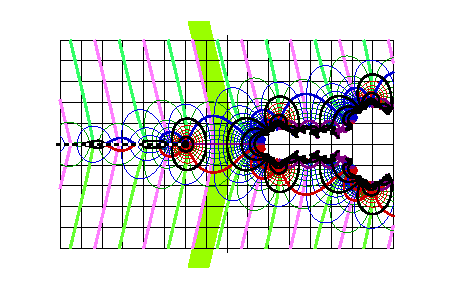
\includegraphics{cauchi/figvladi02a}}
\put(  1,111){\sx{.6}{$\Im(z)$}}
\put(  7, 99){\sx{.58}{$4$}}
\put(  7, 89){\sx{.58}{$3$}}
\put(  7, 79){\sx{.58}{$2$}}
\put(  7, 69){\sx{.58}{$1$}}
\put(  7, 59){\sx{.58}{$0$}}
\put(  2, 49){\sx{.58}{$-1$}}
\put(  2, 39){\sx{.58}{$-3$}}
\put(  2, 29){\sx{.58}{$-3$}}
\put(  2, 19){\sx{.58}{$-4$}}
\put(  2,  9){\sx{.58}{$-5$}}
\put(170,4){\sx{.6}{$\Re(z)$}}
\put(150,4){\sx{.6}{$6$}}
\put(130,4){\sx{.6}{$4$}}
\put(110,4){\sx{.6}{$2$}}
\put( 90,4){\sx{.6}{$0$}}
\put( 66,4){\sx{.6}{$-2$}}
\put( 46,4){\sx{.6}{$-4$}}
\put( 26,4){\sx{.6}{$-6$}}
%\put(12,115){\rot{-70}{\sx{.6}{$\Im(f)\!=\!L$}}\ero }
\put( 38,115){\rot{-77}{\sx{.4}{$\Im(f)\!=\!\Im(L)$}}\ero }
\put( 50,115){\rot{-77}{\sx{.4}{$\Re(f)\!=\!\Re(L)$}}\ero }
\put( 62,115){\rot{-77}{\sx{.4}{$\Im(f)\!=\!\Im(L)$}}\ero }
\put( 98,115){\rot{-77}{\sx{.4}{$\Re(f)\!=\!\Re(L)$}}\ero }
\put(108,115){\rot{-77}{\sx{.4}{$\Im(f)\!=\!\Im(L)$}}\ero }
\put(120,115){\rot{-77}{\sx{.4}{$\Re(f)\!=\!\Re(L)$}}\ero }

\put( 42,14){\rot{77}{\sx{.4}{$\Im(f)\!=\!-\!\Im(L)$}}\ero }
\put( 53,14){\rot{77}{\sx{.4}{$\Re(f)\!=\!\Re(L)$}}\ero }
\put( 65,14){\rot{77}{\sx{.4}{$\Im(f)\!=\!-\!\Im(L)$}}\ero }

\put( 81, 8){\rot{ 76.7}{\sx{.66}{$\mathrm{arctet}(G)$}}\ero }
\end{picture}}

\sx{2.4}{\begin{picture}(320,125)
%\put(0,0){\includegraphics{../cauchi/figslogG}}
%\put(0,0){\includegraphics{cauchi/figslogG}}
\put(-10,0){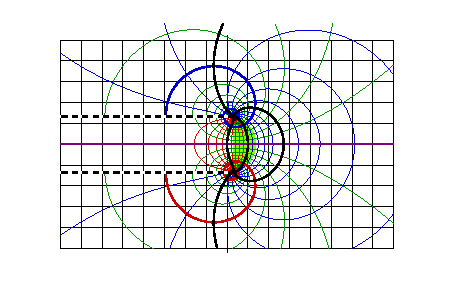
\includegraphics{cauchi/figvladi02b}}
\put( 1,112){\sx{.6}{$\Im(z)$}}
\put( 7, 99){\sx{.58}{$4$}}
\put( 7, 89){\sx{.58}{$3$}}
\put( 7, 79){\sx{.58}{$2$}}
\put( 7, 69){\sx{.58}{$1$}}
\put( 7, 59){\sx{.58}{$0$}}
\put( 2, 49){\sx{.58}{$-1$}}
\put( 2, 39){\sx{.58}{$-2$}}
\put( 2, 29){\sx{.58}{$-3$}}
\put( 2, 19){\sx{.58}{$-4$}}
\put( 2,  9){\sx{.58}{$-5$}}

\put(170,4){\sx{.6}{$\Re(z)$}}
\put(150,4){\sx{.6}{$6$}}
\put(130,4){\sx{.6}{$4$}}
\put(110,4){\sx{.6}{$2$}}
\put( 90,4){\sx{.6}{$0$}}
\put( 66,4){\sx{.6}{$-2$}}
\put( 46,4){\sx{.6}{$-4$}}
\put( 26,4){\sx{.6}{$-6$}}
\put( 95,57){\sx{1}{$G$}}

\put( 46,120){\sx{.4}{$\Re(f)\!=\!2.2$}}
\put( 80,120){\sx{.4}{$\Re(f)\!=\!2$}}
\put(106,120){\sx{.4}{$\Im(f)\!=\!0.6$}}
\put(136,120){\sx{.4}{$\Im(f)\!=\!0.4$}}
\put(171,100){\sx{.4}{$\Im(f)\!=\!0.2$}}
\put(171, 92){\sx{.4}{$\Re(f)\!=\!1.8$}}
\put(172, 60){\sx{.4}{$\Im(f)\!=\!0$}}
\end{picture}}
\end{center}
\caption{functions $f=\mathrm{tet}(z)$ and $f=\mathrm{arctet}(z)$ in the complex 
$z$-plane. \label{figsexpG} }
\end{figure}

% %\newcommand \JP {{}}
% \newcommand \ve {\varepsilon}
% %\subsection{Asymptotics of cauchi-tetration at large imaginary part of the argument}
% \subsection{Expansion of the Cauchy-tetrational at fixed point $L$}
% FOr simplicity, here we consider the only case of base $b=\mathrm e$.
% Asymptotically, the cauchy-tetrational $F$ can be written as follows:
% \begin{align}
% F(z)=\Phi_0(\ve)+
% %\sum_{m=0}^M \beta_n \ve \exp(2 \pi \mathrm{i} m z) \Phi_m(\ve)
% %+\mathcal{O}\!\Big(\ve \exp\big( 2 \pi \mathrm{i} (M+1) z\big) \Big)
% \beta_1 \ve \exp(2 \pi \mathrm{i} z) \Phi_1(\ve)
% +\mathcal{O}\!\Big(\ve^2 \exp\big( 4 \pi \mathrm{i} z\big) \Big)
% \label{eq:dima01}
% \end{align}
% where 
% $\ve=\exp(Lz+R)$
% ~,~ parameters $R$ and $\beta_1$ are complex numbers, and $\Phi_0$, $\Phi_1$ are 
% holomorphic functions, expandable in powerseries 
% \begin{align}
% \Phi_m(x)=\sum_{n=0}^N a_{m,n} x^n + \mathcal{O} \Big( x^{N+1} \Big);
% \end{align}
% $a_{0,0}=L$; 
% $a_{0,1}=1$;
% $a_{1,0}=1$;
% %At $\mathrm i \infty $, $F$ should be $L$, so, $a_{0,0}=L$.
% The substitution of (\ref{eq:dima01}) into equation $F(z+1)=\exp(F(z))$
% and the asymptotical expansion at $|\ve|\ll 1$ determines the coefficients $a$.
% The calculation with Mathematica gives
% \begin{align}
% %a_{0,0}&=L\\
% %a_{0,1}&=1\\
% a_{0,2}&=\frac{1/2}{L-1}\\
% a_{0,3}&=\frac{L+2}{6(L-1)^2(L+1)}\\
% a_{0,4}&=\frac{6+6L+5L^5+L^3}{24(L-1)^3(1+L)(1+L+L^2)}\\
% a_{0,5}&=\frac{24+36L+46L^2+40L^3+24L^4+9L^5+L^6}{120(L-1)^4(1+L)^2(1+L+2L^2+L^3+L^4)}\\
% a_{0,6}&=\frac{\!120\!+\!240L+390L^2+480L^4+416L^5+301L^6+160L^7+64L^8+14L^9+L^{10}}
% {720(L-1)^2(1+L^2)(1+L^2)(1+L+L^2)(1+L+L^2+L^3+L^4)}\\
% %a_{1,0}&=1\\
% a_{1,1}&=%\frac{1}{L-1} = 
% 2 a_{0,2}\\
% a_{1,2}&=%\frac{1+L/2}{(L-1)^2(L+1)} =
% 3 a_{0,3}\\
% a_{1,3}&=%\frac{6+6L+5L^5+L^3}{6(L-1)^3(L+1)(L^2+L+1)} = 
% 4 a_{0,4}\\
% a_{1,4}&=%\frac{24+36L+46L^2+40L^3+24L^4+9L^5+L^6}
% %{24(L-1)^2(1+L)^2(1+L+2L^2+L^3+L^4)} = 
% 5 a_{0,5}\\
% a_{1,5}&=%\frac{\!120\!+\!240L+390L^2+480L^4+416L^5+301L^6+160L^7+64L^8+14L^9+L^{10}}
% %{120(L-1)^2(1+L^2)(1+L^2)(1+L+L^2)(1+L+L^2+L^3+L^4)}=
% 6 a_{0,6}
% \end{align}

% The tetration equation by itself does not determine the parameter $R$ and 
% coefficints $\beta$. The order of magintude of constant $R$ can be 
% estimated even without a computer, just from the {\em assumption}
% that
% \begin{align}
% \mathrm{tet}(z)\approx 1+\mathrm{tet}'(z)\approx Lz+\exp(Lz+R)
% \label{appro1}
% \end{align}
% and $\mathrm{tet}'(0)\approx 1$; although the more precise estimate 
% gives $\mathrm{tet}'(0)\approx 1.091767351258322138$~.
% Then, the rough estimate for $R$ can be written as follows:
% \begin{align}
% R\approx \ln(1+z)-Lz
% \label{appro2}
% \end{align}

% For $z=i/2$, this gives 
% \begin{align}
% R
% \approx -L \mathrm{i}/2 + \ln(1+\mathrm{i}/2-L)
% \approx 0.745-1.046 \mathrm{i}
% \label{R2}
% \end{align}
% and for $z=i$, we get the estiamte 
% \begin{align}
% R\approx -L \mathrm{i} + \ln(1+\mathrm{i}-L)\approx 1.064-0.777 
% \mathrm{i}
% \label{R1}
% \end{align}
% Similar estimates can be obtained for $z=0$ and $z=-1/2$.
% Comparing \rf{R2} and \rf{R1}, we may {\em expect} that $R\approx 
% 1\!-\!i~$. 
% The second decimal digit in this estimate is already doubtful, and 
% we cannot guess even a first digit of the coefficient $\beta_1$ with 
% such a physically-brutal treate.
% With better precision, the coefficients $R$ 
% and $\beta_1$ can be 
% evaluated, fitting the 
% Cauchy-tetration; this gives values
% \begin{align}
% R &\approx 1.077961437528 -0.9465409639478 ~\mathrm{i}& \\
% \beta_1&\approx ~ 0.12233177 ~ -0.02366104 ~\mathrm{i} &	
% %\\	\beta_2&\approx ~~ - 0.25 ~~ - ~ 0.27 ~\mathrm{i} &\\
% \end{align}
% We believe, these values approximate the fundamental mathematical constants.

% Local Variables:
% TeX-master: "../main"
% End:


\section{Reduction to known iteration}\label{sec:Change of base}
This method appears in different facets. The common principle is to
reduce the iteration for high bases $b>\eta$ to the known (regular) iteration of
some function, for example to an exponential with base $\le \eta$.

\subsection{Lévy's approach}
To obtain an extended iteration of $e^x$ Lévy proposes in his article
\cite{levy:exponentielle} the reduction to the iteration of
$f(x)=e^x-1$ in the following way: Let $\alpha$ be an Abel
function of the decremented exponential $e^x -1$ (i.e.\ the regular
Abel function at fixed point 0), then the limit
(which exists)
\begin{align*}
  \slog_{e,z}(u) = \lim_{n\to\infty} \alpha(\exp^{[n]}(u)) -\alpha(\exp^{[n]}(z))
\end{align*}
is an $u$-initialized Abel function of $\exp$. This can be easier seen
when inverting the above formula (using the regular iteration $\beta$ of
$e^x-1$):
\begin{align*}
  \spow_e^w(z) = u = \lim_{n\to\infty} \log^{[n]}(\beta^{w}(\exp^{[n]}(z)))
\end{align*}
which we can more easily be seen to satisfy
$\spow^{w_1+w_2}_e(z)=\spow^{w_1}_e(\spow^{w_2}_e(z))$ and
$\spow^{1}(z)=\exp(z)$.

\begin{align*}
  \slog_b(x)&=\slog_a(\mu_{a,b}(x)) = \lim_{n\to\infty} \slog_a(\exp_b^{[n]}(x)) - n\\
  \slog_{a,u}(x)=\slog_b(x)-\slog_b(u)&= \lim_{n\to\infty}
  \slog_a(\exp_b^{[n]}(x))-\slog_a(\exp_b^{[n]}(u))
\end{align*}
 
\subsection{Change of base}
The base observation is that the following limit exists (and is real) for $1<a<b$
and arguments $x\in\R$:
\begin{align}
  \label{eq:changeofbase:limit}
  \mu_{a,b} := \lim_{n\to\infty} \log_a^{[n]}\circ\exp_b^{[n]}
\end{align}
For $1<a<b$ we can make the following assertions:
\begin{enumerate}
\item If $b\le\eta$ 
  \begin{enumerate}
  \item if $x\le b^+$ then $\mu_{a,b}(x)=a^+$ (const.) 
  \item \label{case:b} $\mu_{a,b}$ maps $(b^+,\infty)\mapsto(a^+,\infty)$. 
    It is strictly increasing and infinitely differentiable on
    $(b^+,\infty)$.
  \item $\mu_{b,a}$ maps $(a^+,\infty)\mapsto(b^+,\infty)$ and is the
    inverse function of $\mu_{a,b}$.
  \end{enumerate}
\item If $b>\eta$ 
  \begin{enumerate}
  \item then $\mu_{a,b}$ is strictly increasing, unbounded
    above and infinitely differentiable \cite{Viana:hairs} TODO[covers
    that all bases?].
  \item $\mu_{a,b}$ maps $(-\infty,\infty)\mapsto ((a,b)^+,\infty)$
    where $(a,b)^+:=\log_a(\mu_{a,b}(0))$; $\mu_{a,b}(0)>0$; $(a,b)^+\ge a^+$ if $a\le\eta$.
  \item $\mu_{b,a}$ maps $((a,b)^+,\infty)\mapsto (-\infty,\infty)$ and
    is the inverse function of $\mu_{a,b}$.
  \end{enumerate}
\item $\mu_{a,b}\circ \mu_{b,c} = \mu_{a,c}$ for $1<a<b<c$, $b>\eta$.
\end{enumerate}
We call it base change because it obviously satisfies
\begin{align}
  \label{eq:changeofbase:relation}
  \mu_{a,b}\circ \exp_b &= \exp_a \circ\mu_{a,b}.
\end{align}
It is however not yet known whether this function is analytic. And
despite the author's conjecture that it is nearly nowhere analytic, we
mention this method here as we consider it an important idea.

If we got an Abel function $\slog_a$ of $a^x$ (for example by regular
iteration at the lower fixed point in the case $a\le\eta$) then we have
also the Abel function $\slog_b$ of $b^x$, $b>a,\eta$, given by:

\begin{align}\label{eq:superchange}
  \slog_b&=\slog_a\circ\mu_{a,b} &\sexp_b&=\mu_{b,a}\circ\sexp_a
\end{align}

\subsection{Walker's approach}
\newcommand{\logi}{\operatorname{logi}}
\begin{align*}
  \log_a\log_a\exp_b\exp_b(x)&=\frac{\ln b}{\ln a}x + \underbrace{\frac{\ln \ln b -
    \ln \ln a}{\ln a}}_{c_{a,b}}=:\tau(x)\\
  \tau^{-1}(a^{\tau(x)})&=\frac{\ln a e^{x\ln(b) + \ln \ln b - \ln \ln
      a}-\ln \ln b + \ln \ln a}{\ln b}
  \\&=b^x+\frac{\ln\ln a-\ln\ln b}{\ln b} = b^x + c_{b,a}
  \\\tau^{-1}(\log_a(\tau(x)))&=\log_b(x-c_{b,a})=:\logi_{b,a}(x)
  \\\log_a^{[n]}\circ\exp_b^{[n]}&= \tau\circ \logi_{b,a}^{[n-2]}\circ
  \exp_b^{[n-2]}
\end{align*}
\subsection{Numerics}
Repeated exponentiation quickly exhaust the range of floating point
numbers. For example for $b=e$, $x=1/8$ there are at most 4 iterations
presentable in extended floating point:
$\exp^{[4]}(1/8)\approx 4.9\times 10^{9}$. For other numbers like $x=1/16$ we can
obtain 5 iterations in extended floating point arithmetics:
$\exp^{[5]}(1/16)\approx 7.7\times 10^{33555749}$. 

So we try to avoid taking too much exponentiations. We do this by not
using the formula $\mu_{a,b,n}=\log_{a}^{[n]}\circ \exp_b^{[n]}$ but save two
iterations by using TODO[ref above]:
\begin{align*}
  \mu_{a,b,n}(x) =\tau(\logi_{b,a}^{[n-2]}(\exp_b^{[n-2]}(x))).
\end{align*}
The precision of $\mu_{a,b}(x)$ is limited to the maximal number $n$ of
iterations of $\exp_b$ that is presentable in the floating point
arithmetic. For example at most 4 iterations are possible in the case
$x=1/8$, which reaches an accuracy of at most
$\mu_{\eta,e,6}(1/8)-\exp_\eta(\mu_{\eta,e,6}(\log(1/8)))=\mu_{\eta,e,6}(1/8)-\mu_{\eta,e,5}(1/8)\approx
8.65\times 10^{-13}$ for $a=\eta$ which is not even ``double'' 
precision. For $x=1/16$ however 5 iterations are presentable in
extended floating point arithmetics which gives a nearly exact result. 

\subsection{Incompatibilities with the other methods}

\subsubsection{Incompatibility with regular iteration}
Looking at equation \eqref{eq:superchange} one might ask whether
$\slog_b$ is the regular superlogarithm (up to an additive constant) if $\slog_a$ is.
For the appropriate bases $b\in(1,\eta]$ case \ref{case:b} applies and so $\slog_a$
must be defined on $(a^+,\infty)$. This is
not the case for the regular superlogarithm at the {\em lower} fixed point,
however it is the case for the regular superlogarithm $\ruslog_a$ at
the {\em upper} fixed point $a^+$! So we concretize our question to:
Is \begin{align*}\ruslog_b(x) - \mu_{a,b}(\ruslog_a(x))\end{align*} a constant function for all $a,b\in
(1,\eta]$? And the answer is ``no'', as the graph of this
quantity shows in figure \ref{fig:muregdiff}. The deviation from a
constant is small, however the picture show the typical extending
oscillation one would expect for different Abel functions. If we have
two Abel functions $\alpha_1$ and $\alpha_2$ then
$\theta=\alpha_1\circ \alpha_2^{[-1]}-\id$ is an 1-periodic function and we can
express the difference as
$\alpha_2-\alpha_1=(\theta+\id)\circ\alpha_1-\alpha_1=\theta\circ\alpha_1$. This
is an oscillating function with ``extending period''. One full
oscillation takes place in each interval $(x,f(x))$, in
our case this is the interval $(x,b^x)$. For example in the picture
you can see the two maxima at $x\approx 5.27$ and $4^{5.27/4}\approx
6.2$ or the two minima at $x\approx 5.65$ and $4^{5.65/4}\approx 7.1$.
\begin{figure}
\begin{center}
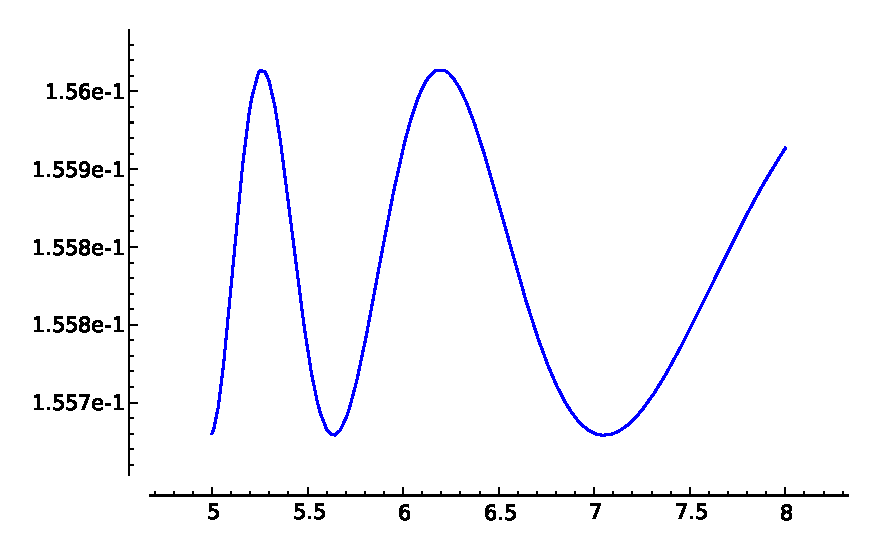
\includegraphics{muregdiff-4-8}
\end{center}
\caption{$y=\ruslog_b(x) - \mu_{a,b}(\ruslog_a(x))$ for $a=8^{1/8}$,
  $b=4^{1/4}=\sqrt{2}$ }
\label{fig:muregdiff}
\end{figure}

\subsubsection{Incompatibility with intuitive iteration}
TODO $\ruslog_\eta \circ \mu_{\eta,e}\neq \islog$ 

\subsubsection{Incompatibility with Cauchy iteration}
TODO $\mu_{e,\eta}\circ \rusexp_\eta\neq \ksexp$ 

%\subsection{Levenstein's Method}

\section{Summary}
%\begin{table}
\begin{tabular}{l|c|c|c|c}
Method & Section & Base $b$ & PS devel.\ & Outcome\\ \hline
Regular ($0<\abs{f_1}\neq 1$, PS) &\ref{sec:Non-parabolic powerseries}& $<\eta$ & at FP & iterate\\ \hline
Regular ($0<\abs{f_1}<1$, limit) &\ref{sec:Non-parabolic limit}& $<\eta$ & - & Schr\"oder, also
iterate\\ \hline
Regular ($f_1=1$, PS) &\ref{sec:Parabolic powerseries}& $=\eta$ & at FP & iterate\\ \hline
Regular ($f_1=1$, limit) &\ref{sec:Parabolic limit}& $=\eta$ & - & Abel\\ \hline
Matrix Power &\ref{sec:Matrix power}& - & everywhere & iterate\\ \hline
Newton/Lagrange &\ref{sec:NewtonLagrange}& $\le \eta$ & - & iterate\\ \hline
% Generalized Antidifference & \\ \hline
Kneser's &\ref{sec:Kneser}& $>\eta$ & - & Abel \\ \hline
Intuitive Abel &\ref{sec:Intuitive Abel}& - & at non-FP & Abel \\ \hline
Cauchy integral &\ref{sec:Cauchy integral}& $>\eta$ & - & super\\ \hline
Change of base &\ref{sec:Change of base}& $>\eta$ & - & super\\ \hline
%Levenstein's & $\eta$ &
\end{tabular}

%\caption{
PS = power series, FP = fixed point, bases are always
greater 1
%}
%\end{table}

\appendix
\section{Closed Form of the Real Fixed Points of the Exponentials}
%TODO move this before the first reference of \sfrt
\begin{wellknown}[real fixed points of exponentials]
  \label{wk:exponential:fixedpoint:real}
  The real function $f(x)=b^x$ has exactly 2 fixed points
  for $1<b<\eta$, exactly one fixed point for $b=\eta$ and no
  fixed point for $b>\eta$. $b\tet n$ converges to the lower real
  fixed point in the case $1<b\le \eta$ and to infinity for $b>\eta$.
\end{wellknown}

A fixed point $z_0$ satisfies $b^{z_0}=z_0$, or equivalently
$b=\sqrt[z_0]{z_0}$.
This solution versus $b$ is shown in figure \ref{figLb}.
\begin{figure}

\begin{center}
\sx{2}{\begin{picture}(270,70)
%\put(0,0){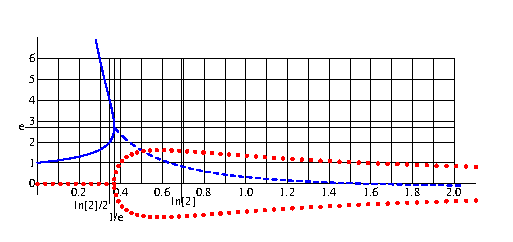
\includegraphics{cauchi/figLb}}
\put(0,0){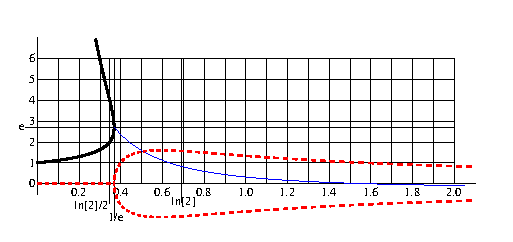
\includegraphics{cauchi/fig02a}}
\put(41,85){\sx{.8}{$z_0$}}
\put(91,36){\sx{.8}{$\Im(z_0)$}}
\put(91,25){\sx{.8}{$\Re(z_0)$}}
\put(220,14){\sx{.66}{$\ln b$}}
\end{picture}}

\end{center}
\caption{\label{figLb}
Solutions $z_0$ of equation $b^{z_0}=z_0$ versus $\ln (b)$, thick solid 
curve  shows two solutions at
$\ln(b)<1/\rm e$. The thin curve shows the real part of the solution at 
$\ln(b)>1/\rm e$.
Dashed curve shows the imaginary part of two solutions, $z_0$ and $z_0^*$. 
\iL{fig02}
}
\end{figure}
To compute $z_0$ directly we would use the inverse
function of $x^{1/x}$. However in most computer algebra systems this
function is not implemented, but instead we have the Lambert $W$
function. We use this occasion to investigate the relation
of the functions self root, self power and multiplied exponential:
\newcommand{\sfpw}{\operatorname{sp}}
\newcommand{\xexp}{M}
\begin{align*}
  &\sfrt(x)=x^{1/x}=\sqrt[x]{x}&&\sfpw(x)=x^x&&\xexp(x)=xe^x\\
  &\sfrt\colon (0,\infty)\to (0,\eta]& &\sfpw\colon (0,\infty)\to
[1/\eta,\infty)&& \xexp\colon (-\infty,\infty)\to [-1/e,\infty)\\
  &\sfrt(e)=\eta\mt{(max)}& &\sfpw(1/e)=1/\eta\mt{(min)} & &\xexp(-1)=-1/e\mt{(min)}
\end{align*}
and their inverses. All these functions have exactly one local and at
the same time global extremum (see figure \ref{fig:3plots}), 
\begin{figure}
  \centering
  \includegraphics[scale=0.8]{realfp/sr}
  \includegraphics[scale=0.8]{realfp/sp}
  \includegraphics[scale=0.8]{realfp/me}
  \caption{The functions $y=\sqrt[x]{x}$, $y=x^x$ and $y=x e^x$.}
  \label{fig:3plots}
\end{figure}
so there is always a strictly decreasing and a strictly
increasing inverse function, which we want to denote by $f^{-1}_-$ and
$f^{-1}_+$ respectively. 
\begin{align*}
  &\sfrt^{-1}_+\colon (0,\eta]\to (0,e]&
  &\sfpw^{-1}_+\colon [1/\eta,\infty)\to [1/e,\infty)&
  &W_+\colon [-1/e,\infty)\to[-1,\infty)\\
  &\sfrt^{-1}_-\colon (1,\eta]\to [e,\infty)&
  &\sfpw^{-1}_-\colon [1/\eta,1)\to (0,1/e]&
  &W_{-}\colon [-1/e,0)\to (-\infty,-1]
\end{align*}

Each function is analytically conjugate to each other in the following way:
\begin{align*}
  \sfrt(x)&=1/\sfpw(1/x)&\sfpw(x) &= \exp(\xexp(\ln(x))) &
  \xexp(x)&=\ln(\sfpw(\exp(x)))\\
  \sfrt(x)&=\exp(-\xexp(-\ln(x))) & \sfpw(x) &= 1/\sfrt(1/x) &
  \xexp(x) &= -\ln(\sfrt(\exp(-x)))
\end{align*}
Accordingly the inverse functions can be defined:
\begin{align*}
  \sfrt^{-1}_\pm(x)&=1/\sfpw^{-1}_\pm(1/x)&
  \sfpw^{-1}_\pm(x) &= \exp(W_\pm(\ln(x))) &
  W_\pm(x)&=\ln(\sfpw^{-1}_\pm(\exp(x)))\\
  \sfrt^{-1}_\pm(x)&=\exp(-W_\pm(-\ln(x))) &
  \sfpw^{-1}_\pm(x) &= 1/\sfrt_\pm^{-1}(1/x) &
  W_\pm(x) &= -\ln(\sfrt_\pm^{-1}(\exp(-x)))
.\end{align*}
We see that
each of self root, self power and multiplied exponential
can serve as a base function, whose inverse can be used to define the
inverses of the other functions.
As far as we know of these only the inverse of the multiplied
exponential (the Lambert $W$ function)
is implemented in standard computer algebra systems. Its branches are
indexed equally in these systems and correspond to 
$W_\pm$ in the following way:
\begin{center}
\begin{tabular}{l|c|c|c}
            & Maple{\texttrademark} &  Mathematica{\texttrademark}    & Sage{\texttrademark}  \\\hline
  $W_+(z)=$ & LambertW(0,z) & ProductLog[0,z] & mpmath.lambertw(z,0)\\
  $W_-(z)=$ & LambertW(-1,z) & ProductLog[-1,z] &
  mpmath.lambertw(z,-1)
\end{tabular}
\end{center}
\begin{wellknown}\label{wk:fixedpoint:formula}
  The lower fixed point $b^-\in (0,e]$ for $b\in(0,\eta]$ and the upper
  fixed point $b^+\in [e,\infty)$ for $b\in(1,\eta]$ of $b^x$ are
  respectively given by
  \begin{align}
    b^\pm&=\sfrt^{-1}_\mp(b) = 1/\sfpw^{-1}_\mp(1/b)=\exp(-W_\mp(-\ln(b)))
    = \frac{W_\mp(-\ln(b))}{-\ln(b)}
  .\end{align}
  The derivative at the fixed points is
  \begin{align}
    \exp_b'(b^\pm) = \ln(b^\pm) = -\ln(\sfpw^{-1}_\mp(1/b)) = -W_\mp(-\ln(b))
  .\end{align}
\end{wellknown}
\begin{proof}
  The last part of the first equation is due to
  $e^{-W(y)}=\frac{W(y)}{y}$.
  The first part of the second equation:
  $\exp_b'(b^\pm)=\ln(b)\exp_b(b^\pm)=\ln(b)b^\pm = \ln(b^\pm)$.
\end{proof}
The most famous fixed point pair is probably $(2,4)$ for $b=\sqrt{2}$.
\section{The complex fixed points of exponentials}
\begin{figure}
%\begin{picture}(530,440)\sx{.9}{
\begin{picture}(530,400)\sx{.9}{
\put(0,0){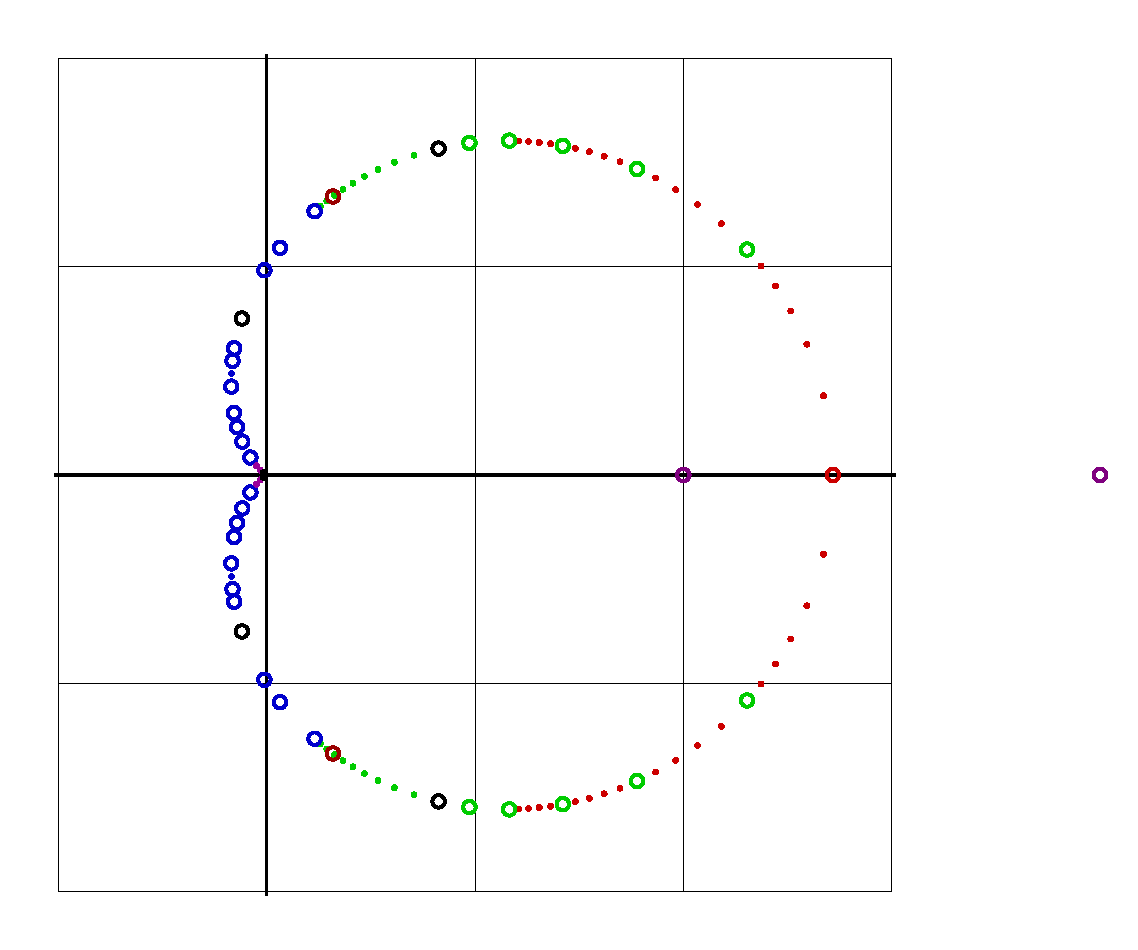
\includegraphics{cauchi/fig02b}}
\put( -6,405){\sx{1.6}{$\Im(p)$}}
\put(  2,316){\sx{1.6}{$1$}}
\put(  2,216){\sx{1.6}{$0$}}
\put( -6,116){\sx{1.6}{$-1$}}
\put( -6, 16){\sx{1.6}{$-2$}}
%
\put(114,346){\sx{1.4}{$b\!=\!3$}}
\put(130,324){\sx{1.4}{$b\!=\!4$}}
\put( 84,316){\sx{1.4}{$b\!=\!5$}}
\put( 70,296){\sx{1.4}{$b\!=\!10$}}
\put( 68,283){\sx{1.4}{$b\!=\!20$}}
\put( 68,272){\sx{1.4}{$b\!=\!30$}}
\put( 58,258){\sx{1.4}{$b\!=\!100$}}
\put( 56,2460){\sx{1.4}{$b\!=\!1000$}}
%
\put(156,348){\sx{1.4}{$b\!=\!\mathrm e$}}
\put(176,381){\sx{1.4}{$b\!=\!2$}}
\put(261,383){\sx{1.4}{$b\!=\!1.7$}}
\put(303,367){\sx{1.4}{$b\!=\!1.6$}}
\put(353,330){\sx{1.4}{$b\!=\!1.5$}}
\put(367,308){\sx{1.4}{$b\!=\!1.48$}}
\put(385,280){\sx{1.4}{$b\!=\!1.46$}}
\put(390,252){\sx{1.4}{$b\!=\!1.45$}}
\put(394,225){\sx{1.4}{$b\!=\!\exp(1/\mathrm{e})$}}
\put(294,225){\sx{1.4}{$b\!=\!\sqrt{2}$}}
\put(490,225){\sx{1.4}{$b\!=\!\sqrt{2}$}}
\put(391,180){\sx{1.4}{$b\!=\!1.45$}}
\put(384,152){\sx{1.4}{$b\!=\!1.46$}}
\put(368,126){\sx{1.4}{$b\!=\!1.48$}}
\put(355,103){\sx{1.4}{$b\!=\!1.5$}}
\put(302, 66){\sx{1.4}{$b\!=\!1.6$}}
\put(261, 48){\sx{1.4}{$b\!=\!1.7$}}
\put(176, 51){\sx{1.4}{$b\!=\!2$}}
\put(156, 86){\sx{1.4}{$b\!=\!\mathrm e$}}
%
\put( 40,210){\sx{1.4}{$b\!=\!1000000$}}
\put( 52,188){\sx{1.4}{$b\!=\!1000$}}
\put( 58,174){\sx{1.4}{$b\!=\!100$}}
\put(108,163){\sx{1.4}{$b\!=\!30$}}
\put( 66,150){\sx{1.4}{$b\!=\!20$}}
\put(113,142){\sx{1.4}{$b\!=\!10$}}
\put( 86,118){\sx{1.4}{$b\!=\!5$}}
\put(131,108){\sx{1.4}{$b\!=\!4$}}
\put(114, 86){\sx{1.4}{$b\!=\!3$}}
%
\put(  8,  0){\sx{1.4}{$-1$}}
\put(117,  0){\sx{1.4}{$0$}}
\put(217,  0){\sx{1.6}{$1$}}
\put(317,  0){\sx{1.6}{$2$}}
\put(401,  0){\sx{1.6}{$\Re(p)$}}
}\end{picture}
\caption{
The primary (nearest to the real axis) fixed points $p$ of $b^x$ in
the complex $p$-plane for various values of $b$. 
%absicssa unity corresponds to the natural tetration ($b\!=\!\rme$).
\iL{fig03}
}
\end{figure}
%Author: Henryk Trappmann, created 20080622

\begin{proposition}
  Let $b>1$ then for each integer $k\ge 2$ there is exactly one solution
  $z$ of $z=b^z$ in the horizontal strip $2\pi
  (k-1)/\ln(b)\le\Im(z)<2\pi k/\ln(b)$. We call this solution
  $b[k]$. More specifically it is
  situated in $2(k-1)\pi/\ln(b) < \Im(z) < (2\pi k -\pi)/\ln(b)$. For $k=1$ we distinguish 3 cases :
  \begin{enumerate}
  \item If $b>e^{1/e}$ then the above is also valid for $k=1$.
  \item
  If $b=e^{1/e}$ then there is exactly one solution for $k=1$,
  this solution is $e=:b[1]$;
  \item
  If $1<b<e^{1/e}$ then there are exactly two solutions
  $b^-<e<b^+=:b[1]$.
  \end{enumerate}
  For each solution $b[j]$, $j\ge 1$, the conjugate is also a
  solution of the equation which we denote by $b[-j]$. There are no
  other solutions than the before mentioned.
\end{proposition}
\begin{proof}
  Let $z=re^{i\alpha}=r(\cos(\alpha)+i\sin(\alpha))$ and let
  $c=\ln(b)$ then the fixed point equation is equivalent to the
  equation system:
  \begin{align}
    r&=e^{cr\cos(\alpha)}\label{eq:radius}\\
    \alpha&=cr\sin(\alpha)\label{eq:angle}
  \end{align}
  Let us now substitute $s=cr$ and assume $\alpha\neq 2\pi m$,
  for any integer $m\ge 0$:
  \begin{align*}
    \ln(s)-\ln(c)=\ln(r) &= s\cos(\alpha)\\
    s&=\frac{\alpha}{\sin(\alpha)}
  \end{align*}
  and substituting the second into the first
  \begin{align*}
    \ln\frac{\alpha}{\sin(\alpha)}-\ln(c) &= \alpha
    \frac{\cos(\alpha)}{\sin(\alpha)}\\
    f(\alpha):=\ln\frac{\alpha}{\sin(\alpha)}-\alpha\cot(\alpha)&=\ln(c)
  \end{align*}
  We show that $f$ is strictly increasing on $2k\pi< \alpha <
  (2k+1)\pi$ for $k\ge 0$ and strictly decreasing for $k<0$ by
  contemplating the sign of its derivative:
  \begin{align*}
    f'(x) &= \frac{\sin(x)}{x}\left( -\frac{x \cos(x)}{\sin(x)^2}
      + \frac{1}{\sin(x)} \right) 
    -\frac{\cos(x)}{\sin(x)} - x\left(-\sin(x)\frac{1}{\sin(x)}
      +\cos(x)\frac{-1}{\sin(x)^2}\cos(x) \right)\\
    &= - 2\cot(x) +\frac{1}{x}+x + x\cot(x)^2 = 
     x+\frac{-2 x \cot(x) + 1 + x^2 \cot(x)^2}{x}\\
    &= x+\frac{(1- x \cot(x))^2 }{x}
  \end{align*}
  The last line is positive for $x>0$ and negative for $x<0$, so there
  can be at most one solution of $f(x)=\ln(c)$ on $x\in(2 k\pi, 2 k\pi + \pi)$
  and there is a solution for $k\neq 0,-1$ because in this case
  $f((2k\pi,(2k+1)\pi))=(-\infty,+\infty)$.
  The imaginary part of $z$ for this solution is $r \sin(\alpha)$
  which is equal to $\alpha/\ln(b)$ by \eqref{eq:angle}, so there is
  exactly one solution in $2k \pi/\ln(b) < \Im(z) < (2\pi(k+1)
  -\pi)/\ln(b)$ for $k\neq 0,-1$.

  Let us now consider the case $k=0$. Here $f((0,\pi))=(-1,\infty)$,
  so if $c>1/e$ then $\ln(c)>-1$ and there is exactly one solution
  $f(x)=\ln(c)$ for $0<x<\pi$. If $\ln(c)\le -1$ then $f(x)=\ln(c)$ has
  no solution in $0<x<\pi$.

  We now consider the case $\alpha=2k\pi$, $k\ge 0$. If $k>0$ then
  \eqref{eq:angle} is invalid. So we consider $\alpha=0$ for which
  equation \eqref{eq:angle} is always valid. In this case only 
  $r=e^{cr}$ has to be satisfied. Now we look for zeros on $0\le
  x<\infty$ of the corresponding $g(x)=e^{cx}-x$. We can determine the
  global minimum $\mu$ at $x$ of this function by 
  \begin{align*}
    0&=g'(x)=ce^{cx}-1\\
    x&=\frac{1}{c}\ln\frac{1}{c}=-\frac{\ln(c)}{c}\\
    g''(x)&=c^2e^{cx}=c^2\frac{1}{c}=c>0\\
    \mu:=g(x)&=\frac{1}{c}(1+\ln(c))
  \end{align*}
  Clearly the minimum $\mu$ is smaller than 0 for $\ln(c)<-1$ and
  equal to $0$ for $\ln(c)=-1$ which corresponds to the last both
  cases $c=\frac{1}{e}$ having one solution and $0<c<\frac{1}{e}$
  having two solutions.
\end{proof}
\begin{proposition}[Repelling and attracting fixed points of $b^z$]
  Let $b>1$, then $\abs{{\exp_b}'(p)}>1$ for all non-real fixed
  points $p$. For the real fixed points in the
  case $1<b<e^{1/e}$ we have 
  \begin{align}
    {\exp_b}'(b^-) &< 1 & {\exp_b}'(b^+)&>1.
  \end{align}
  and ${\exp_b}'(e)=1$ for $b=e^{1/e}$.
\end{proposition}

\begin{proposition}
  Let $b>e^{1/e}$ and let
  \begin{align*}
    \log_{b,k}(z) &:= \frac{\log (z) + 2\pi i k}{\ln(b)}
  \end{align*}
  then for any $k>0$ and $z_0$ in the upper halfplane:
  \begin{align*}
    b[k]&=\lim_{n\to\infty} {\log_{b,k-1}}^{[n]}(z_0)\\
    {\exp_b}'(b[k]) &= \log_{b,k-1}(b[k]).
  \end{align*}
\end{proposition}
The fixed points can in the same way obtained as in knowledge
\ref{wk:fixedpoint:formula} via the branches of $\sfrt$, $\sfpw$ and
Lambert $W$, where the last is most important practically, as Lambert
$W$ is implemented (with its branches) in most computer algebra
systems
\begin{center}
\begin{tabular}{l|c|c|c}
  &Maple{\texttrademark} &Mathematica{\texttrademark} &Sage{\texttrademark}  \\\hline
       $W_k(z)=$ &LambertW(k,z) & ProductLog[k,z]& mpmath.lambertw(z,k)
\end{tabular}
\end{center}
With this branching we obtain for $k\ge 1$
\begin{align}
  &&b[k] &= \frac{W_{-k}(-\ln(b))}{-\ln(b)}&1&<b\\
  b^- &= \frac{W_{0}(-\ln(b))}{-\ln(b)} &
  b^+ &= \frac{W_{-1}(-\ln(b))}{-\ln(b)} & 
  1&<b\le\eta.
\end{align}

% Local Variables:
% TeX-master: "main"
% End:


\bibliographystyle{alpha}
\bibliography{main}
TODO: keywords: 
exp b fixed points,
Kneser Abel function
Matrix power 
3-argument Ackermann function
regular iteration
Schroeder function
fractional iteration formal powerseries

\end{document}
